\section{Visualize S(Q) and G(r)}

As individual runs or post-processed runs are completed, the output files will be placed in their respective directories specified in Table \ref{table_directory_struct}. The S(Q) data is found in the \fileio{SofQ} directory and the real-space data is found in the \fileio{gofr} and \fileio{PDF}. 

To visualize and plot both sets of of data (reciprocal-space and real-space), we use the \guicmd{Calculate G(r)} tab shown below: 

\noindent\makebox[\textwidth]{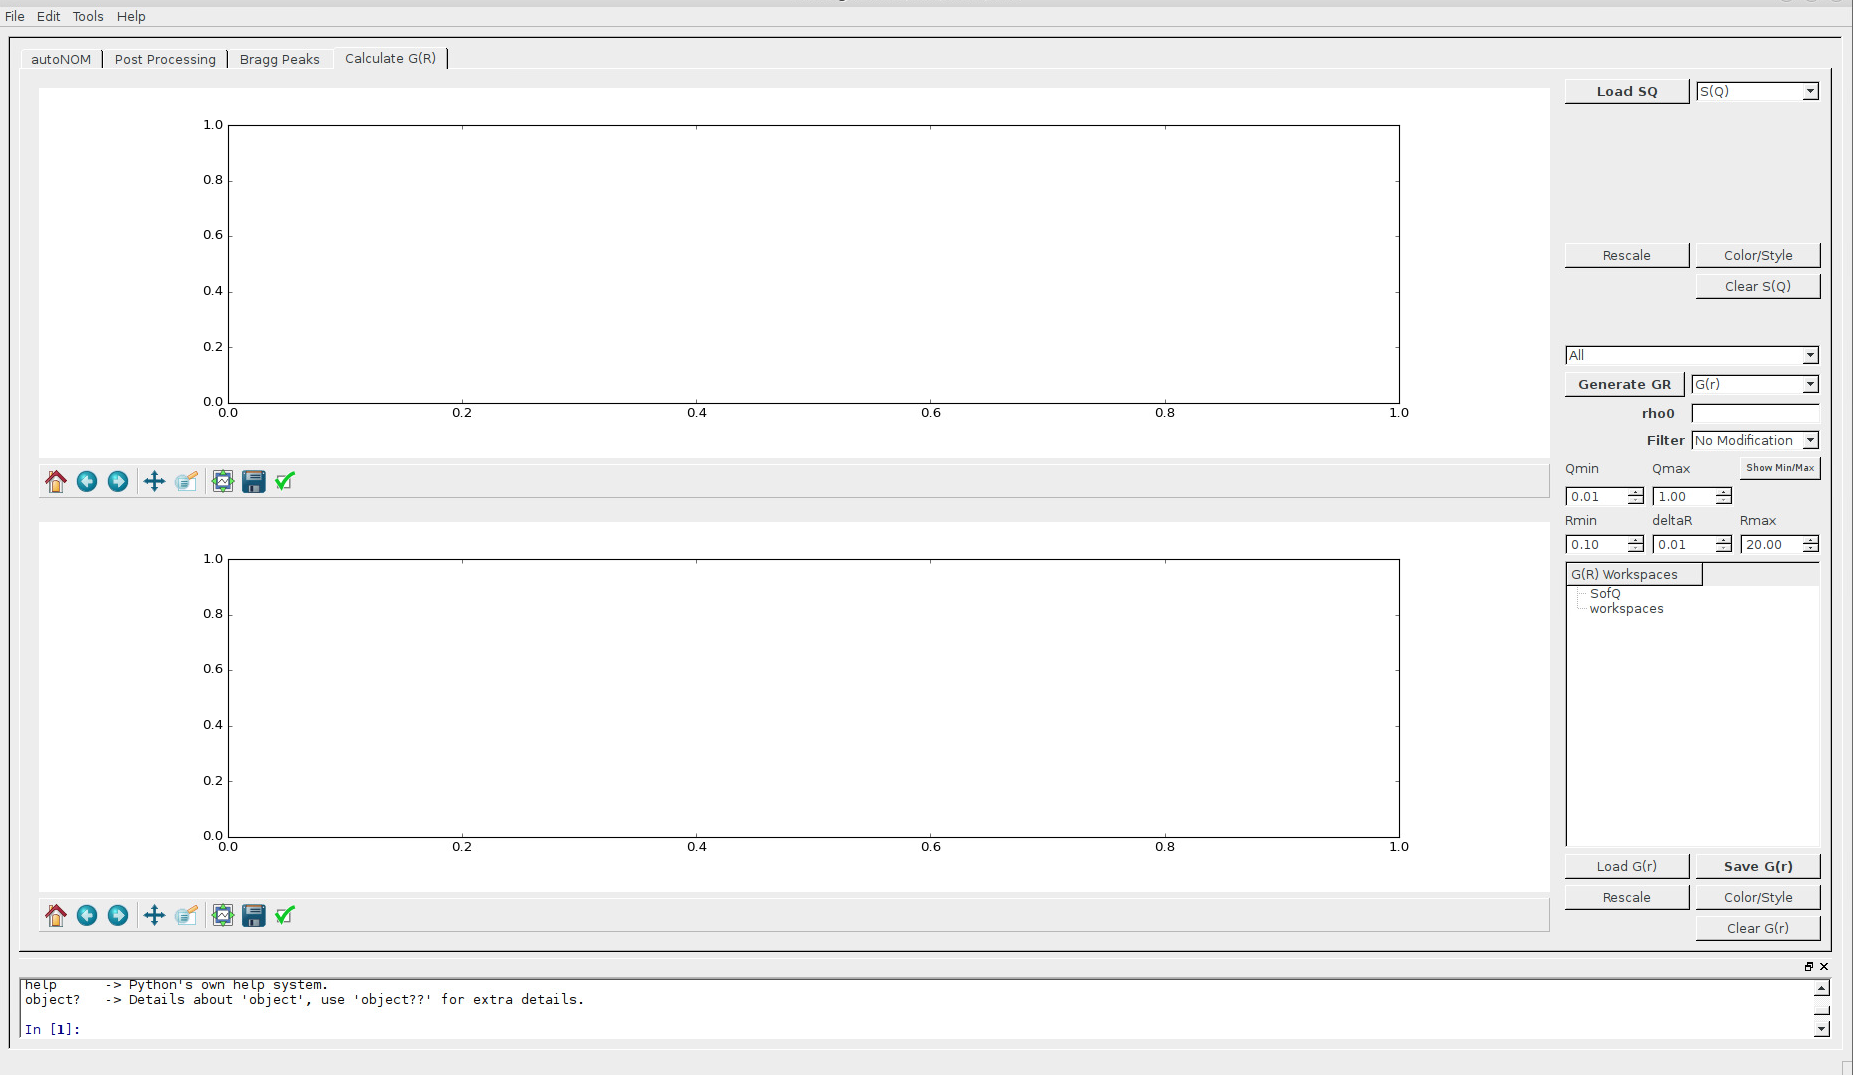
\includegraphics[width=0.9\paperwidth]{graphics/tab4/tab4.png}}

A note on how the two plots work: When S(Q) data is loaded in, the Fourier transform is calculated automatically and the corresponding G(r) is displayed in the corresponding plot. Thus, ADDIE allows one to simultaneously view both the S(Q) and corresponding G(r) and also adjust and refine both datasets in an "on-the-fly" manner.

\subsection{Load S(Q) data}

First load in S(Q) datasests. Go to the top right and press the \guicmd{Load SQ} button. You should be presented with a file dialog similar to the one below:

\noindent\makebox[\textwidth]{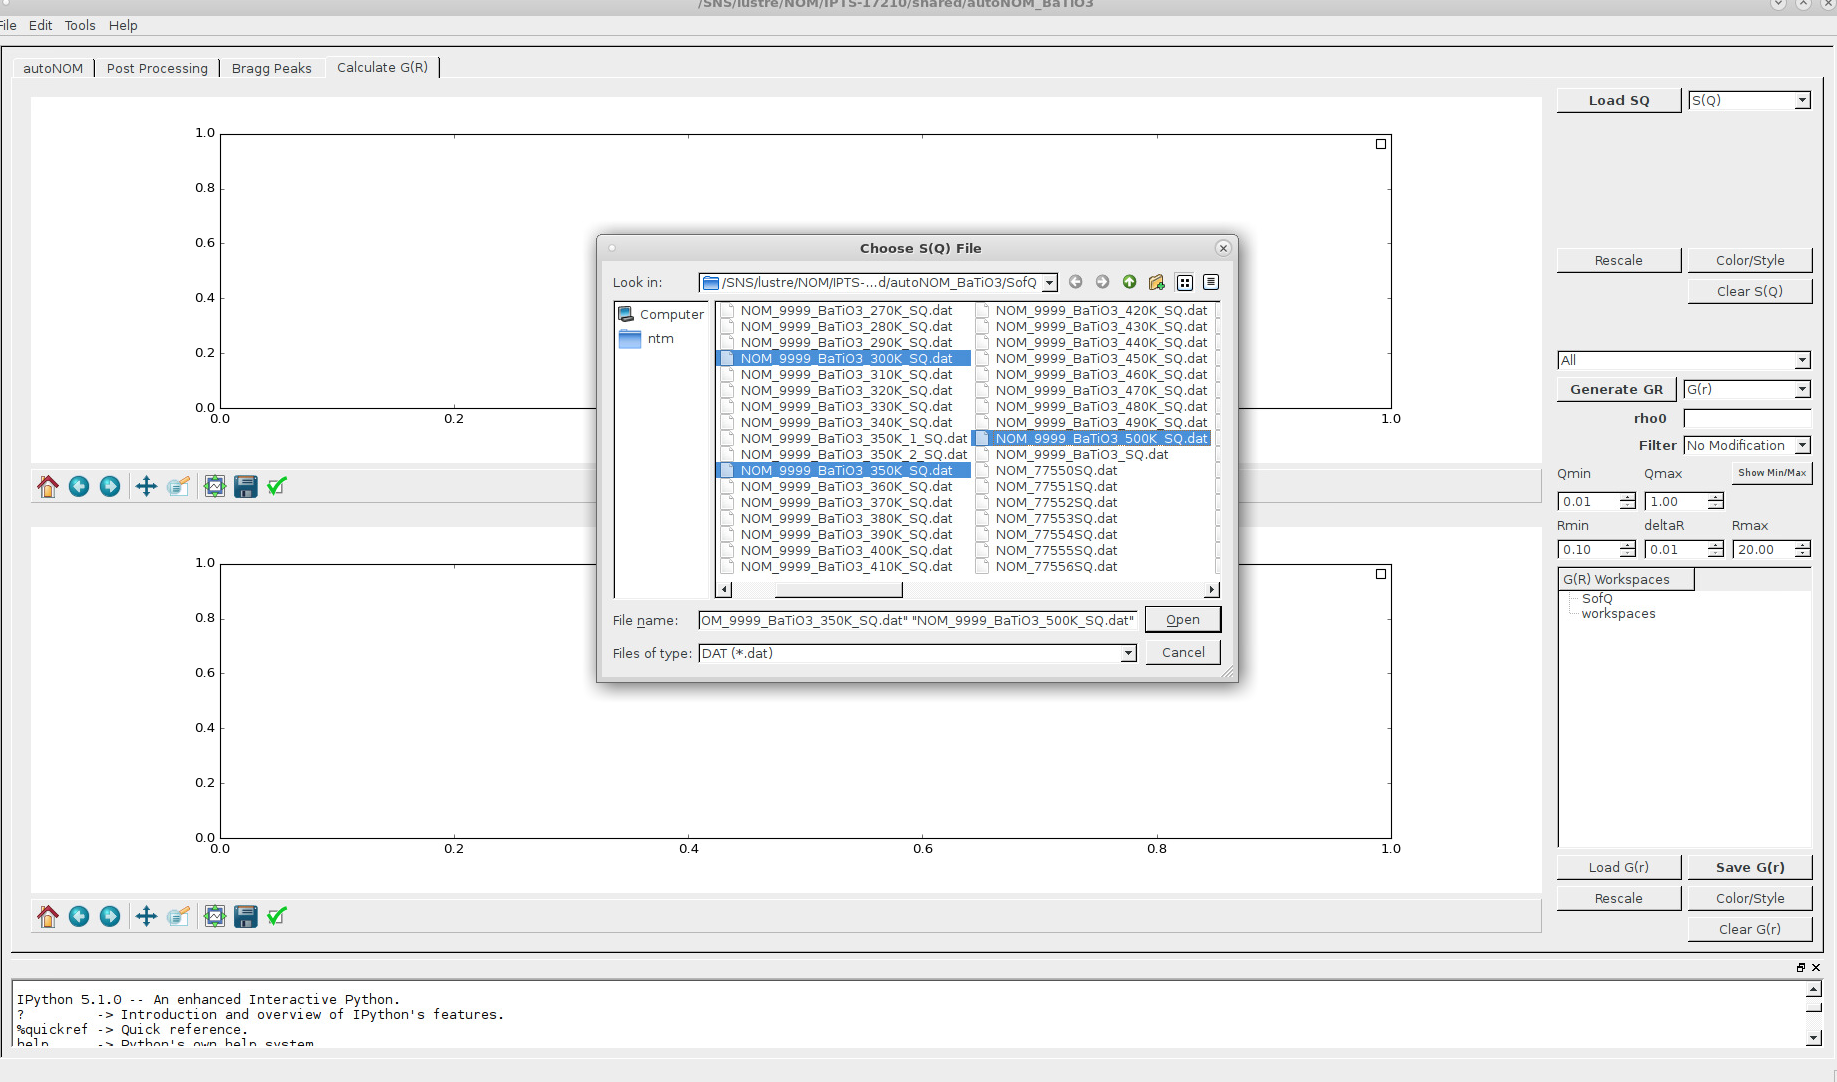
\includegraphics[width=0.9\paperwidth]{graphics/tab4/tab4_loadSQ.png}}

If you are not in the \fileio{SofQ} directory, double-click the \fileio{SofQ} diretory to see the files that are available.  From here, you can select individual runs, labeled as \fileio{NOM\_<run number>SQ.dat} or you can select post-processed runs such as summed files, labeled as \fileio{NOM\_9999\_<given title>\_SQ.dat}.

You can also select multiple individual runs while holding the \cmd{Ctrl} key or you can select a span of runs by holding the \cmd{Shift} key while selecting the runs. Once the runs are selected, press the \guicmd{Open} button. For our example above, we get the following displayed:

\noindent\makebox[\textwidth]{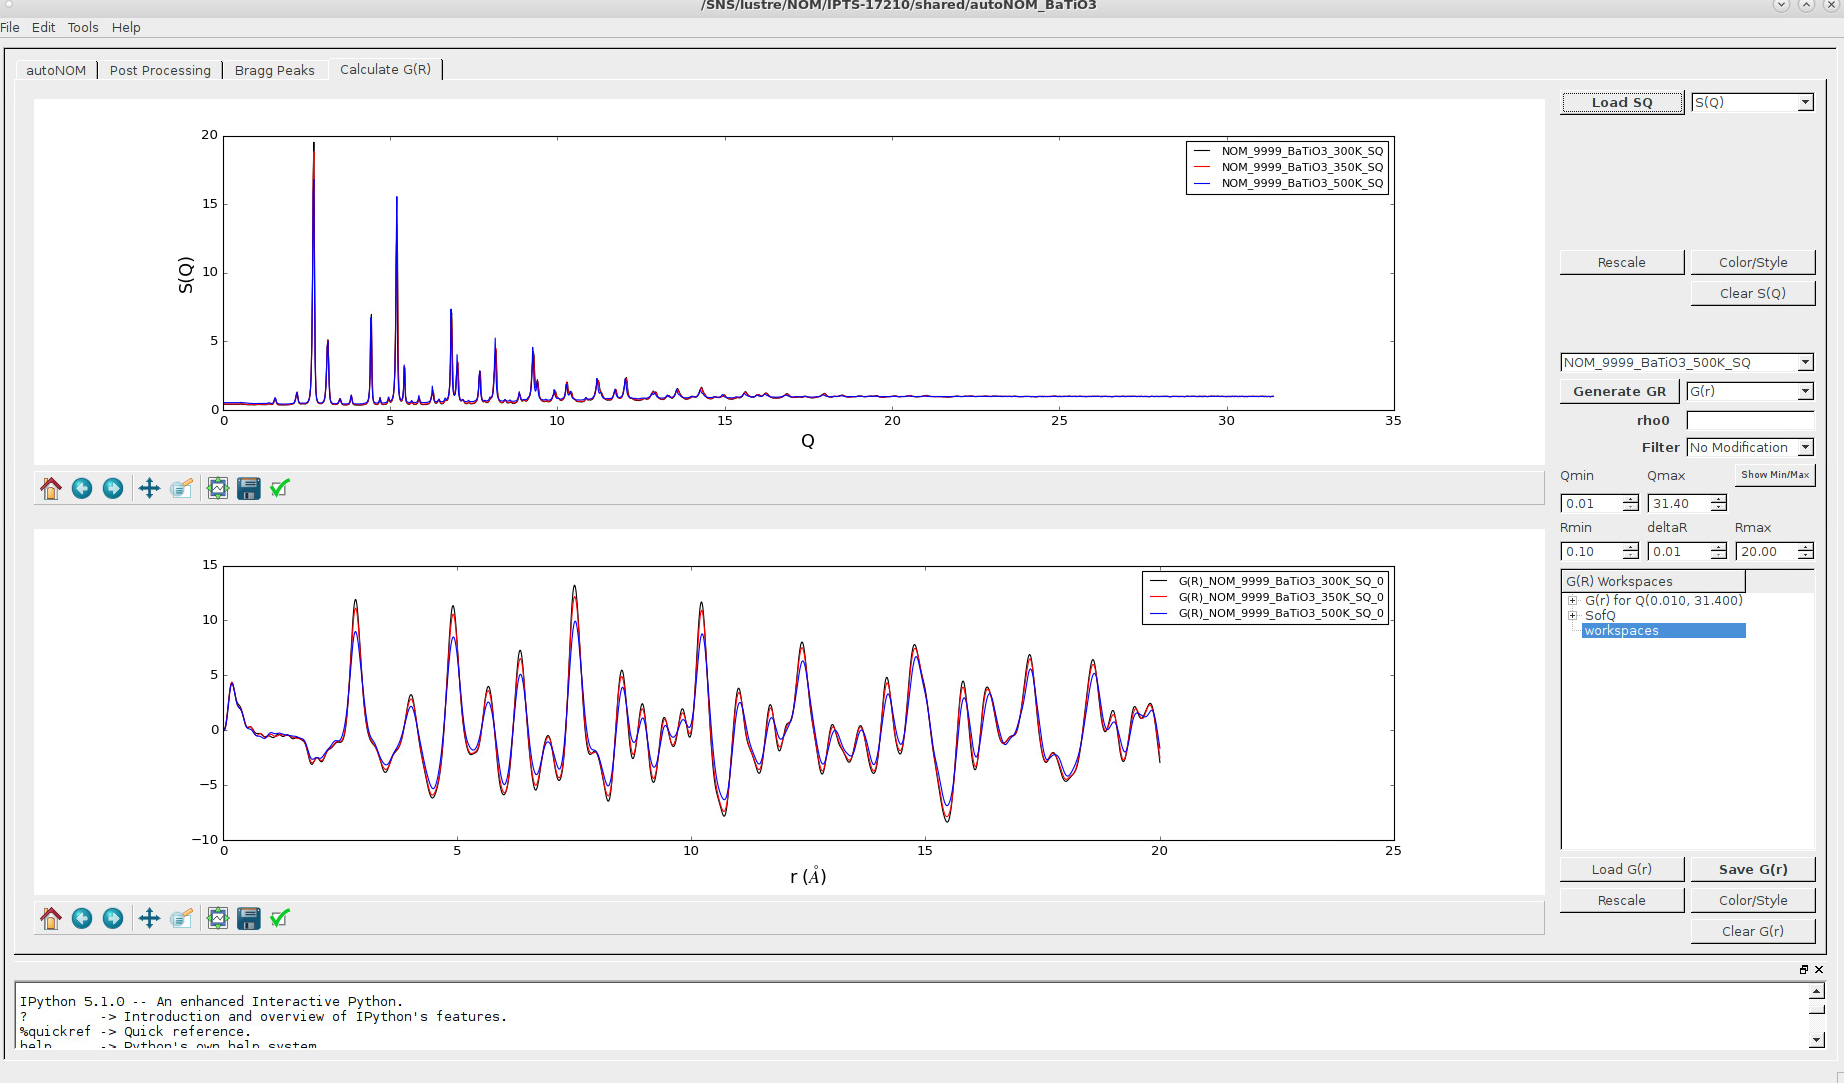
\includegraphics[width=0.9\paperwidth]{graphics/tab4/tab4_loadSQ_afterLoaded.png}}

We can see all three datasets were loaded and the Fourier transform data is displayed as well, based on the current options set for the transform, described more below. 

\subsection{Adjust S(Q) graphs}

On the top right, next to the \guicmd{Load SQ} button, we can change the x-axis of the reciprocal-space plot. We can choose from \guicmd{S(Q)}, \guicmd{S(Q)-1}, and \guicmd{Q[S(Q)-1]}, shown below:

\noindent\makebox[\textwidth]{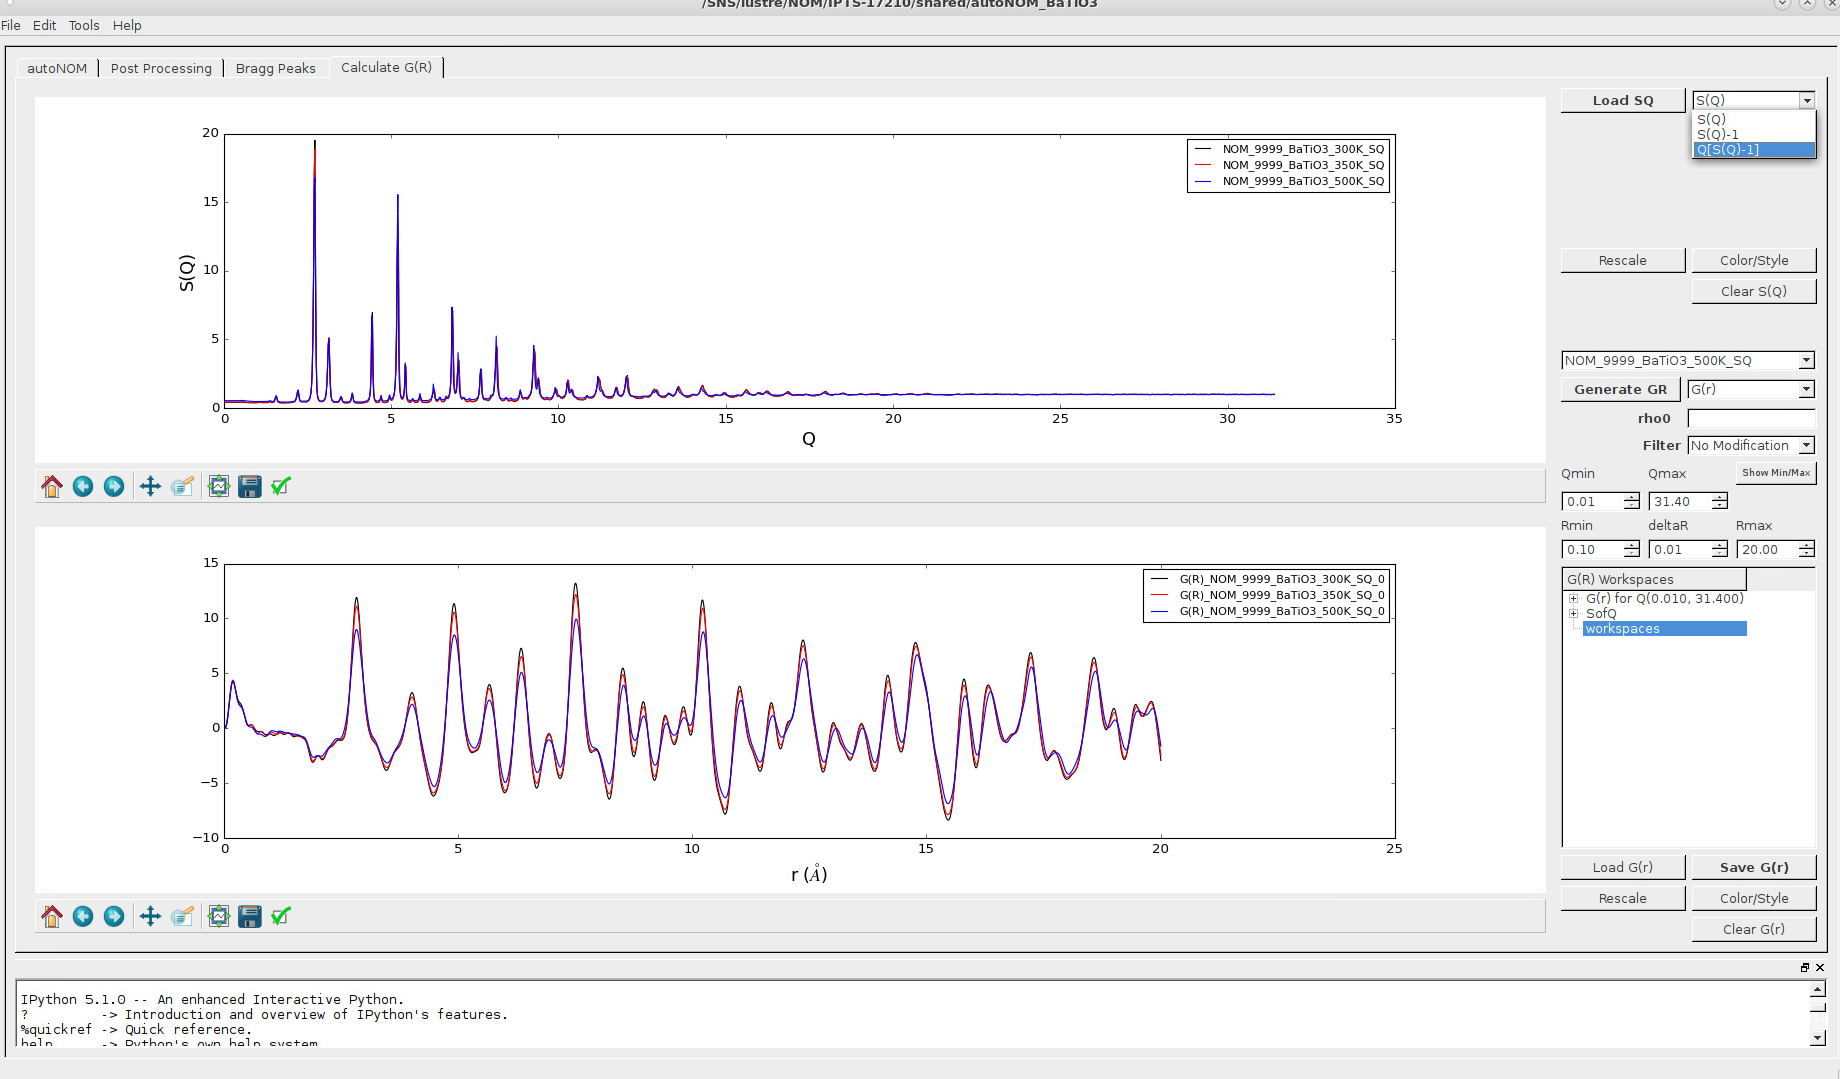
\includegraphics[width=0.9\paperwidth]{graphics/tab4/tab4_populatedGraph_sofqXaxisDropDown.png}}

Selecting the \guicmd{Q[S(Q)-1]} option will produce a plot view like the one below:

\noindent\makebox[\textwidth]{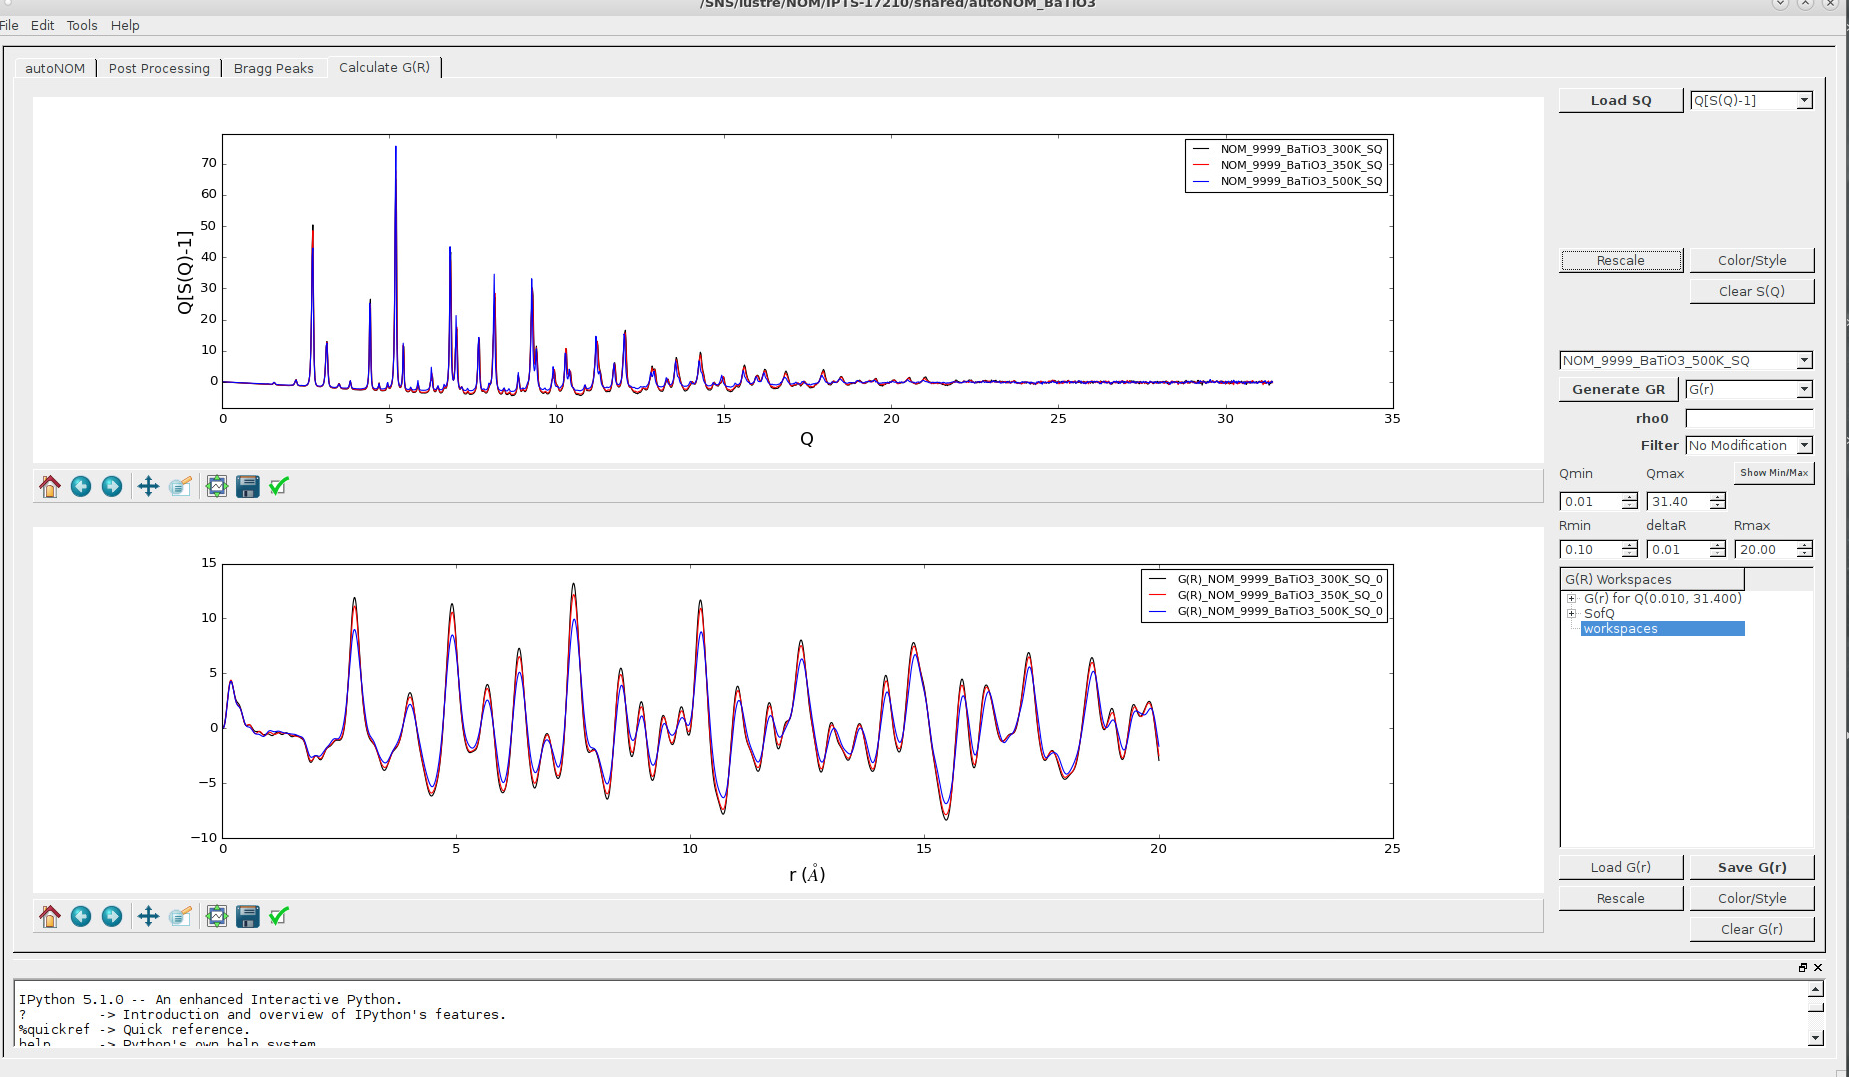
\includegraphics[width=0.9\paperwidth]{graphics/tab4/tab4_populatedGraph_QSofQminus1.png}}

Below this, we have the \guicmd{Rescale} button. If we change the previous drop-down back to \guicmd{S(Q)}, we get the following in the display:

\noindent\makebox[\textwidth]{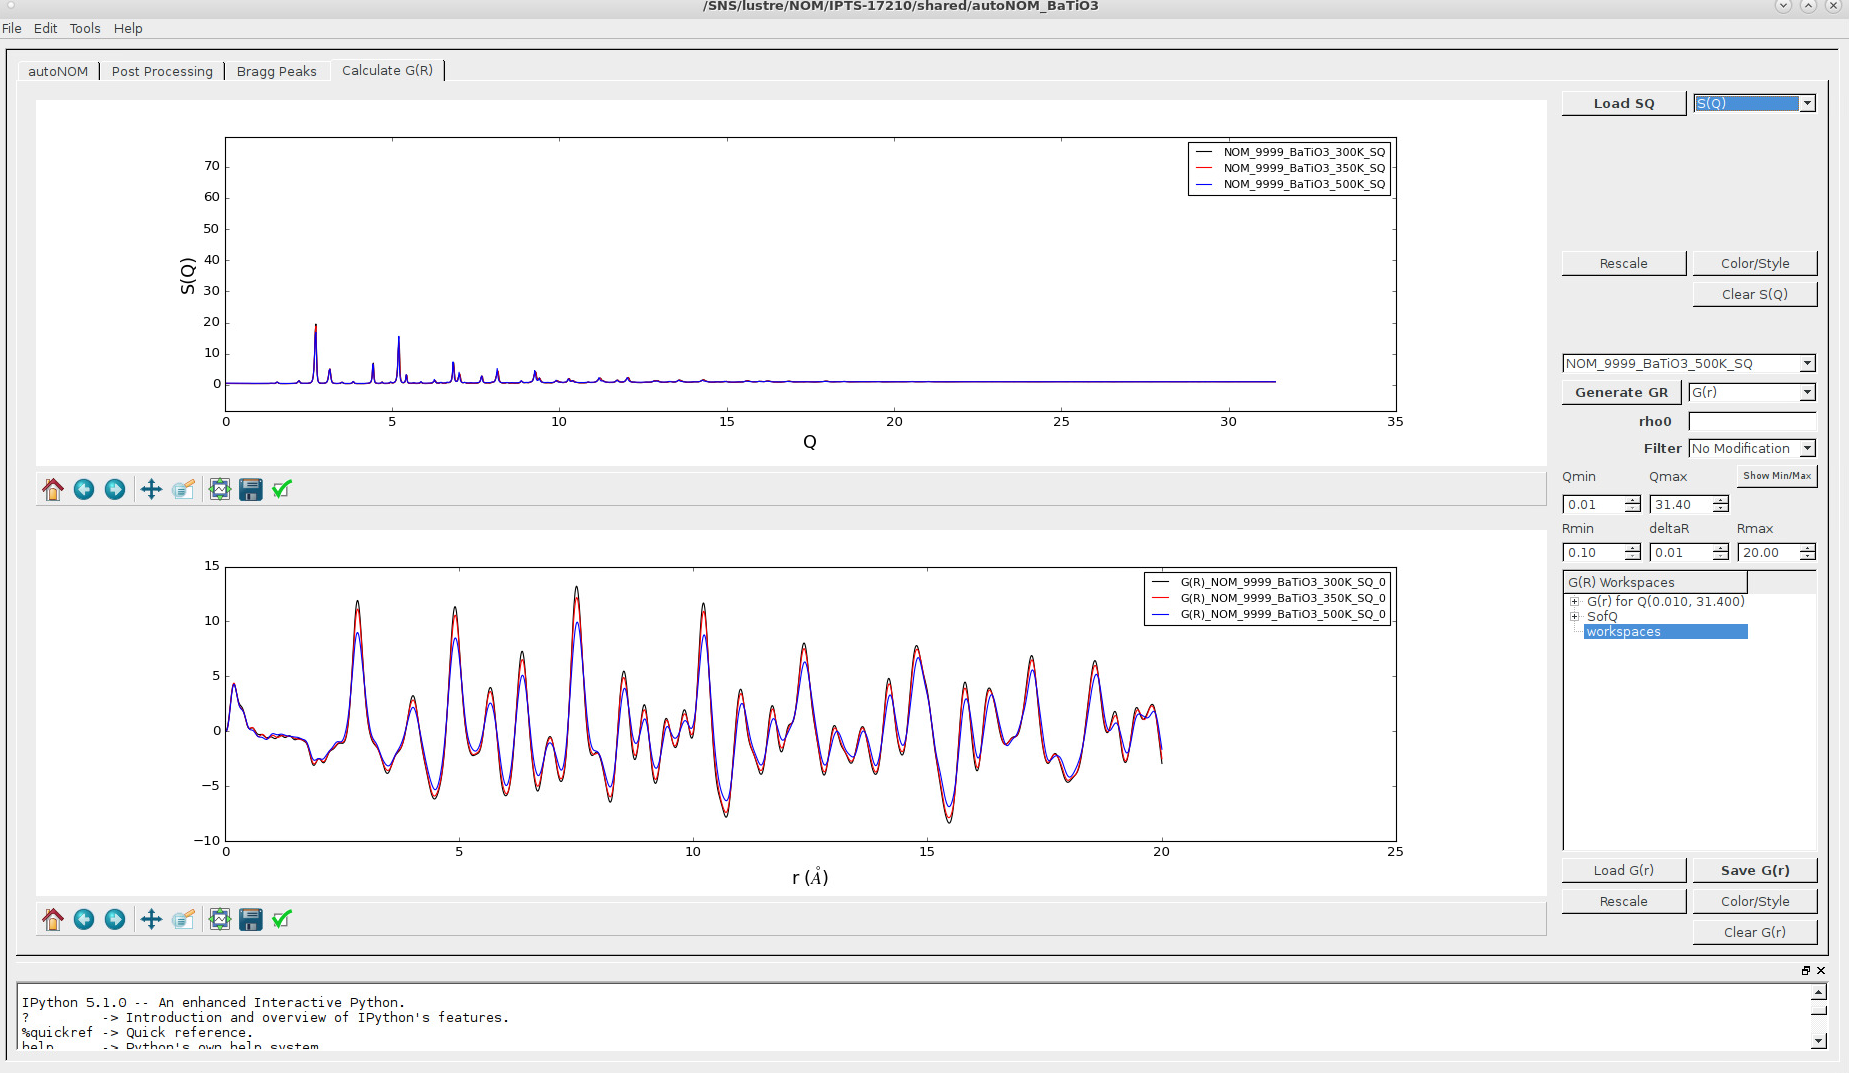
\includegraphics[width=0.9\paperwidth]{graphics/tab4/tab4_populatedGraph_rescaleNeeded.png}}

Clearly, the figure needs to be rescaled to display the data properly. Clicking the \guicmd{Rescale} button, we get back to the previous state for the S(Q) data, as shown below:

\noindent\makebox[\textwidth]{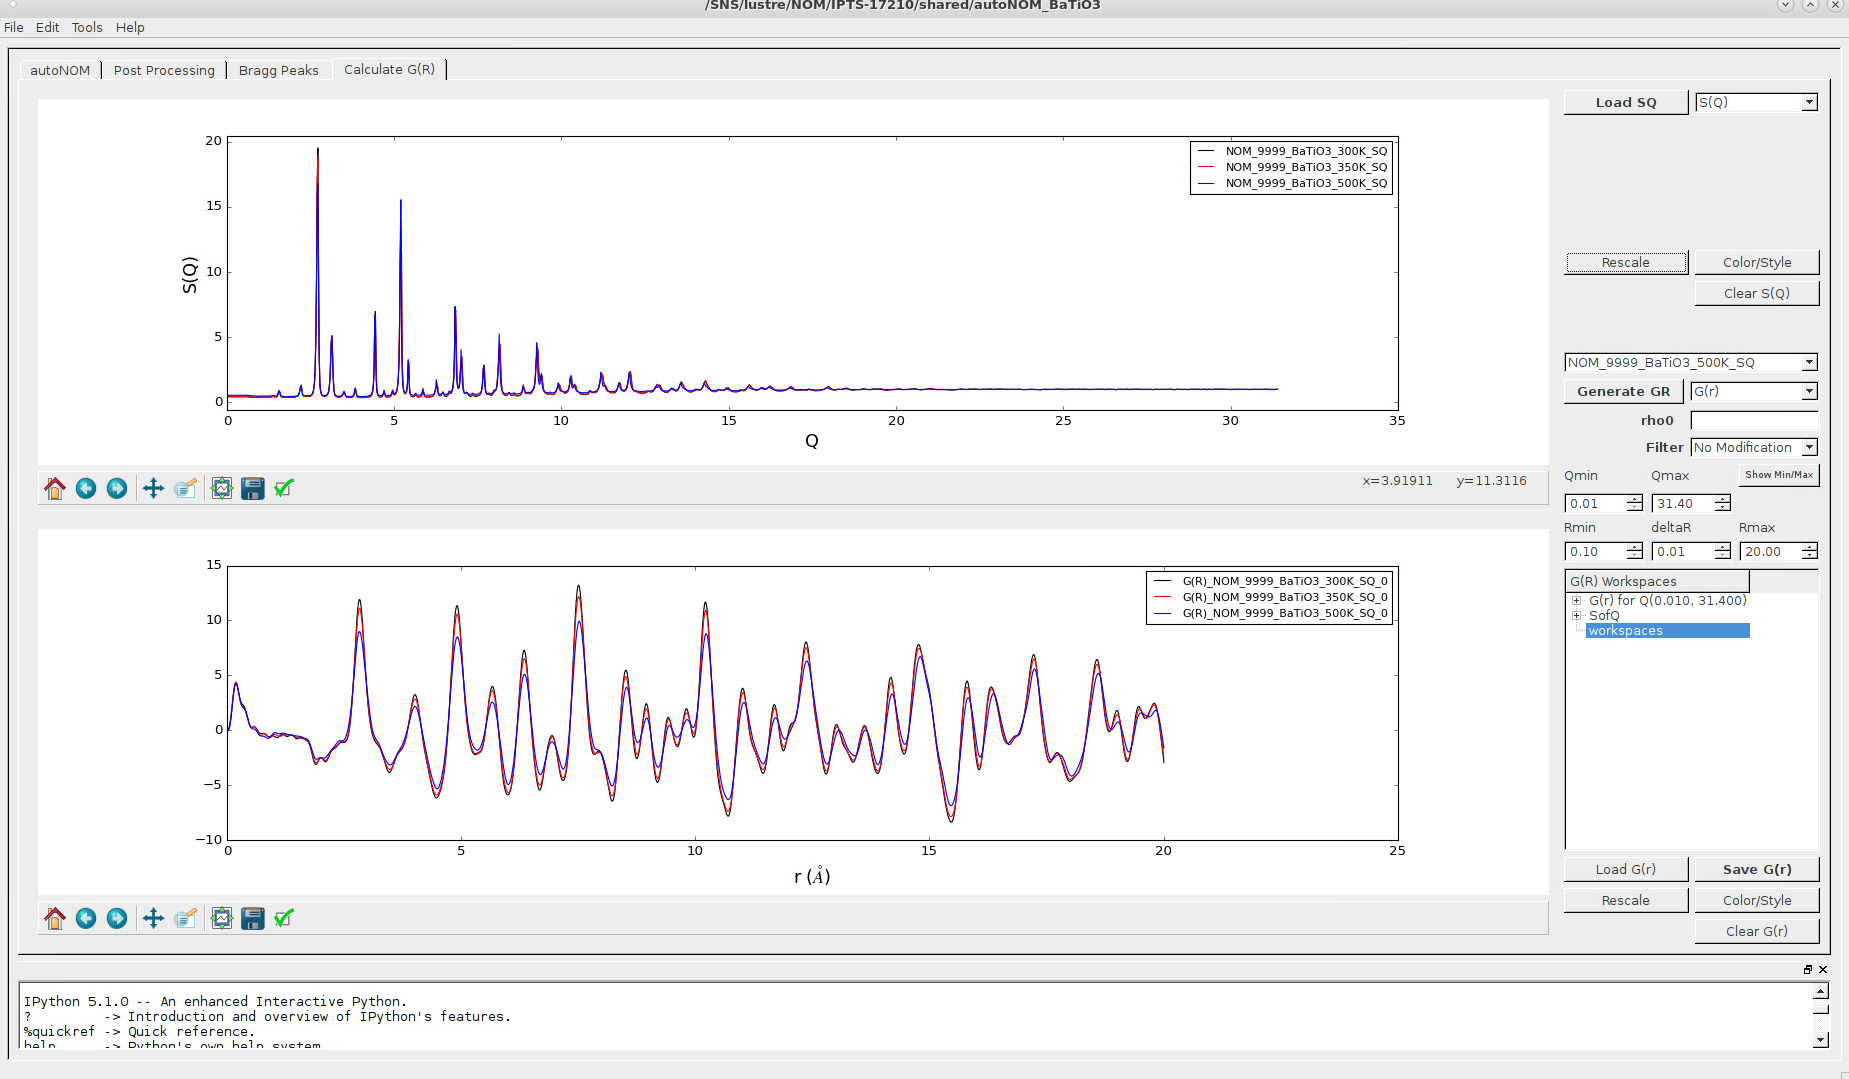
\includegraphics[width=0.9\paperwidth]{graphics/tab4/tab4_populatedGraph_rescaleApplied.png}}

The \guicmd{Color/Style} button can be used to change the display of the S(Q) data in the plot. After pressing the \guicmd{Color/Style} button, we are presented with a file dialog box. We can select the workspace from the drop-down list we would like to change, shown below, and can change the color of the curve, add markers, and select the fill and edge color of the markers from the other drop-downs: 

\noindent\makebox[\textwidth]{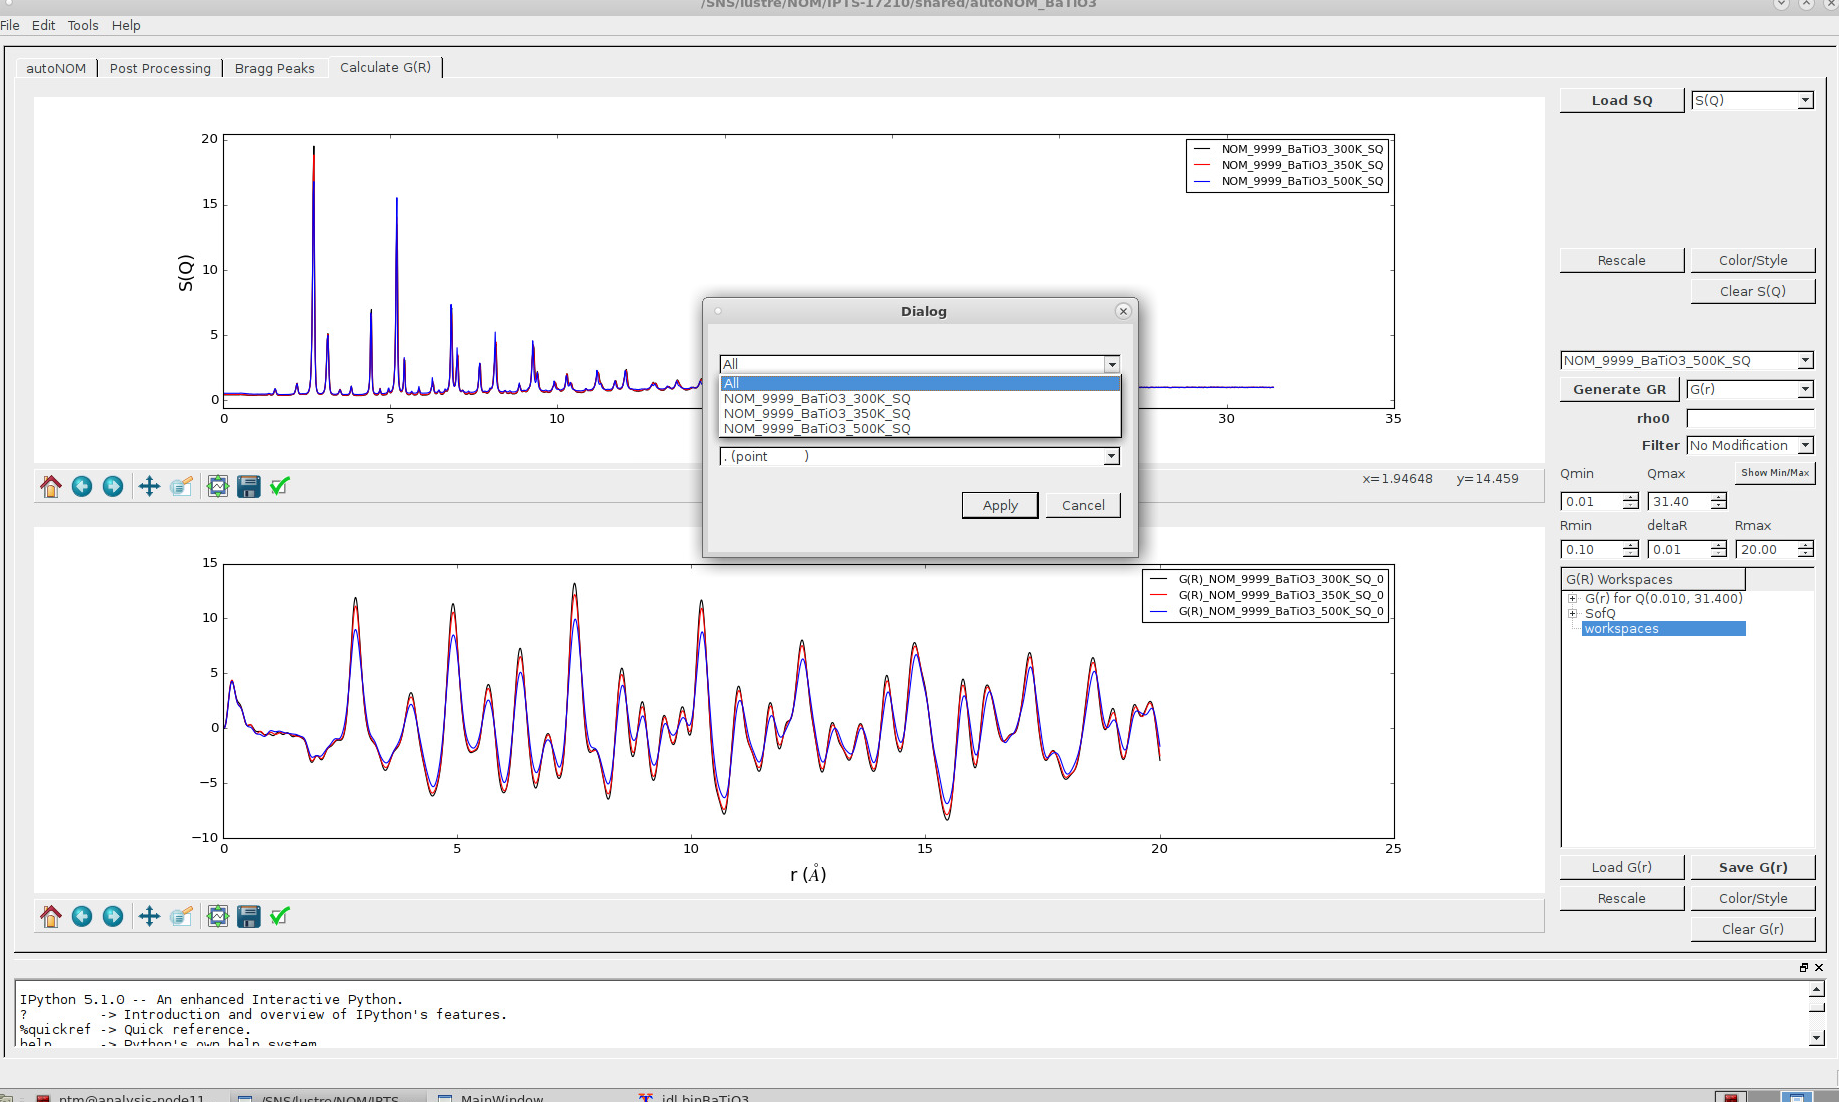
\includegraphics[width=0.9\paperwidth]{graphics/tab4/tab4_populatedGraph_colorStyle.png}}

The \guicmd{CClear S(Q)} button can be used to clear the plotted reciprocal space data sets from the plot view. The datasets are still available to replot in the \guicmd{Workspace Tree}. If we press this from the previous state, we end up with the following below:

\noindent\makebox[\textwidth]{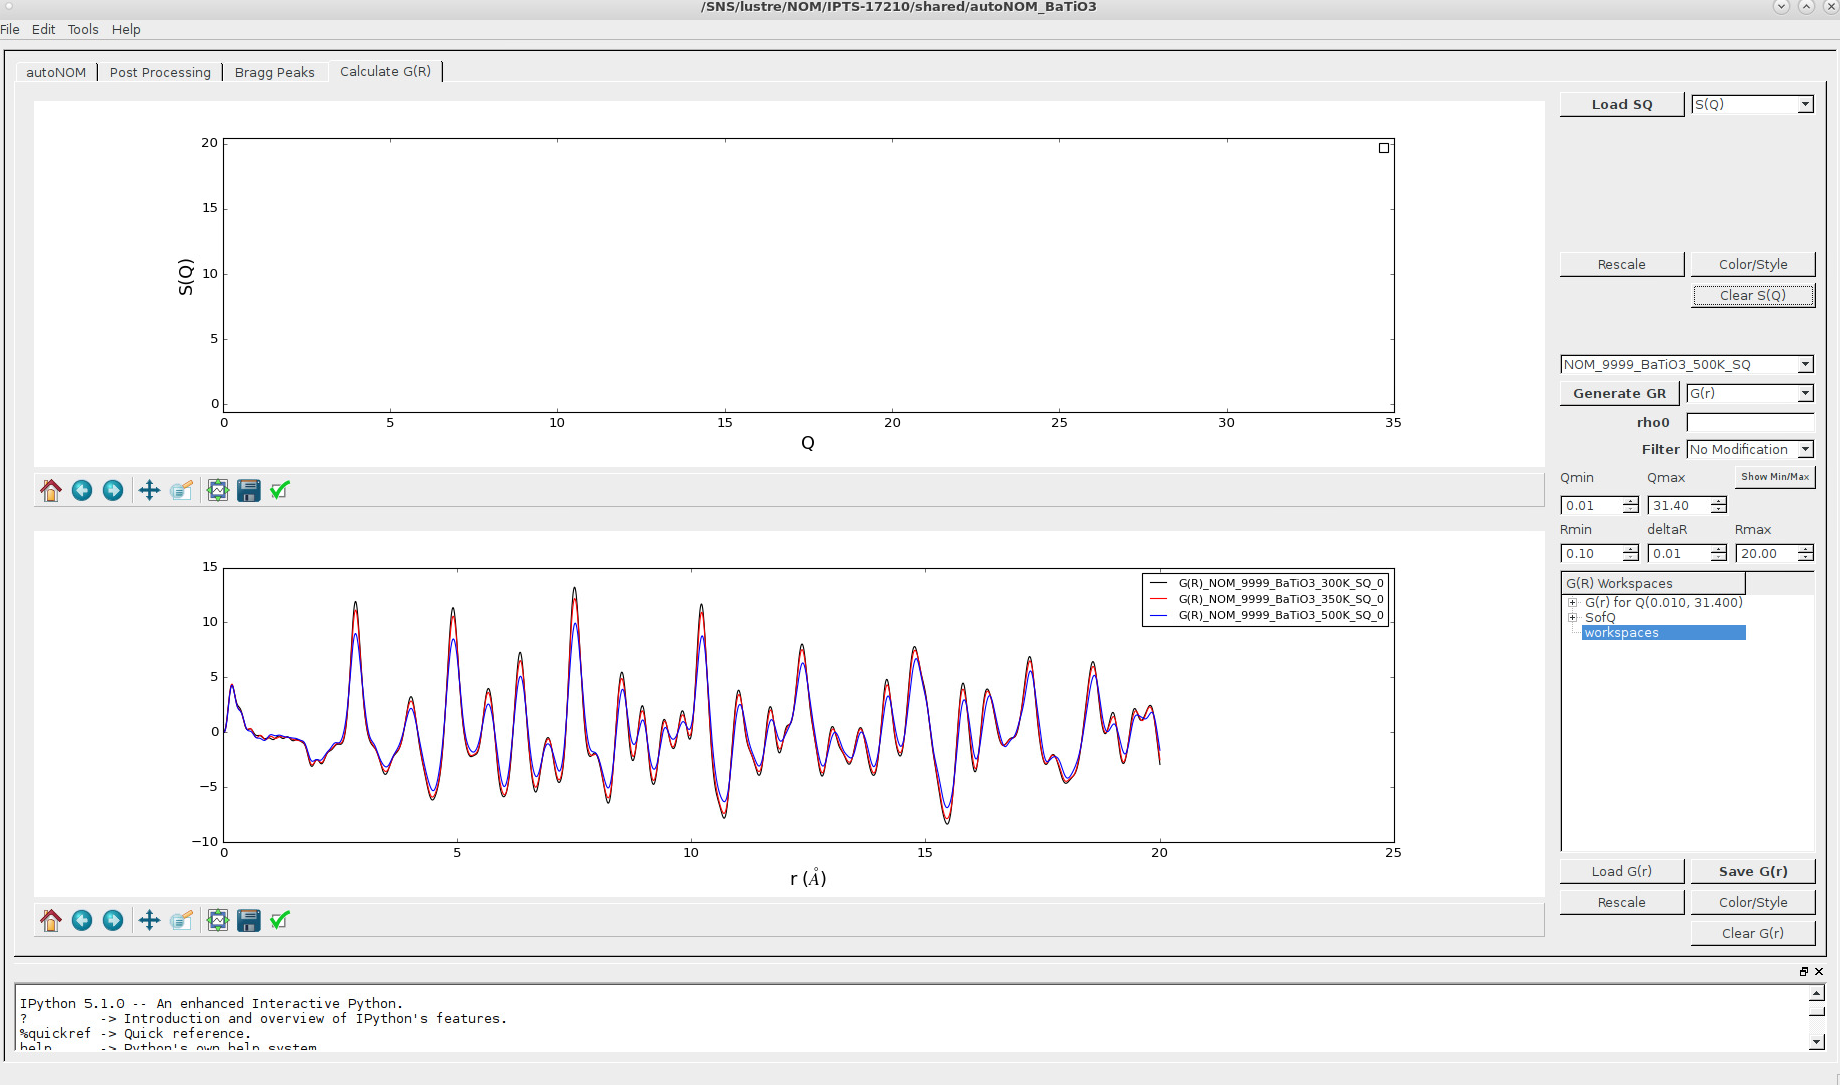
\includegraphics[width=0.9\paperwidth]{graphics/tab4/tab4_populatedGraph_clearSofQ.png}}

In the \guicmd{Workspace Tree}, we can expand the SofQ parent node and see the datasets still available. In the following, we see the datasets are still available even though we cleared the plot view previously:

\noindent\makebox[\textwidth]{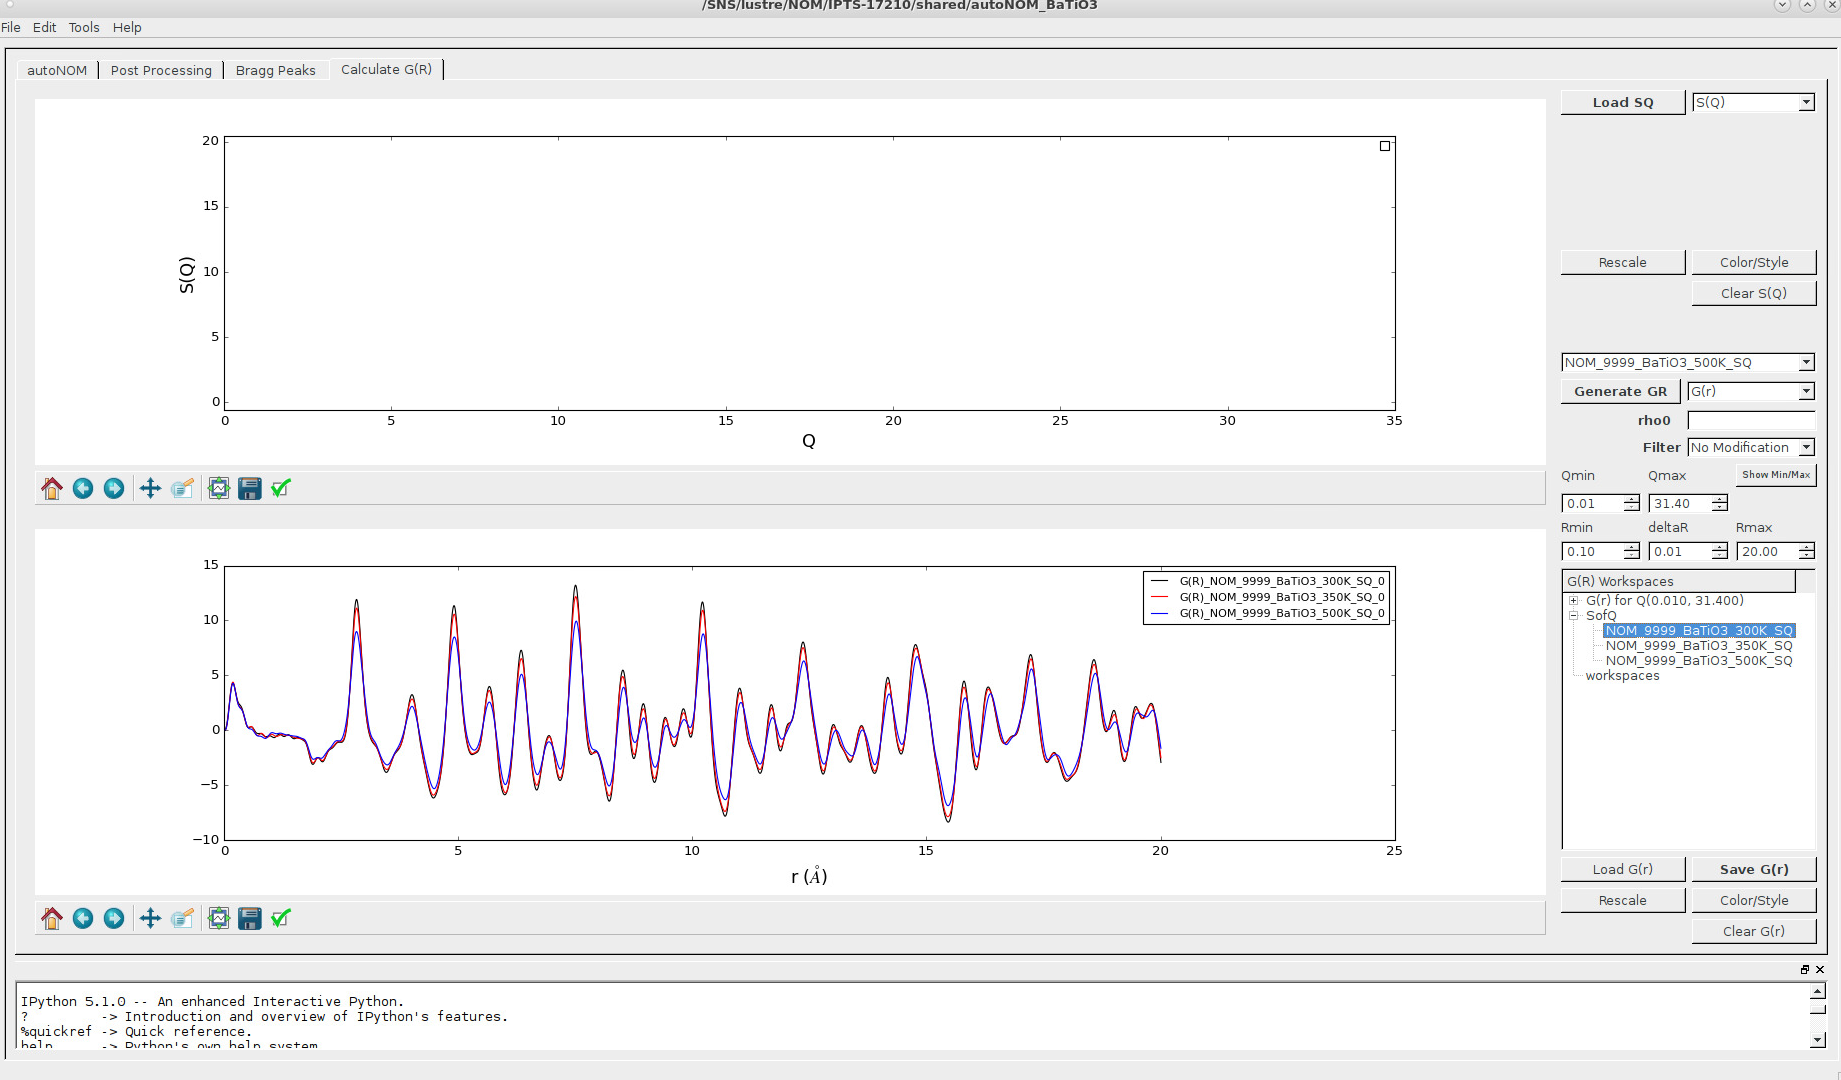
\includegraphics[width=0.9\paperwidth]{graphics/tab4/tab4_populatedGraph_workspaceTree.png}}

Right-clicking any of the data sets in the SofQ workspace tree will give the following options shown below:

\noindent\makebox[\textwidth]{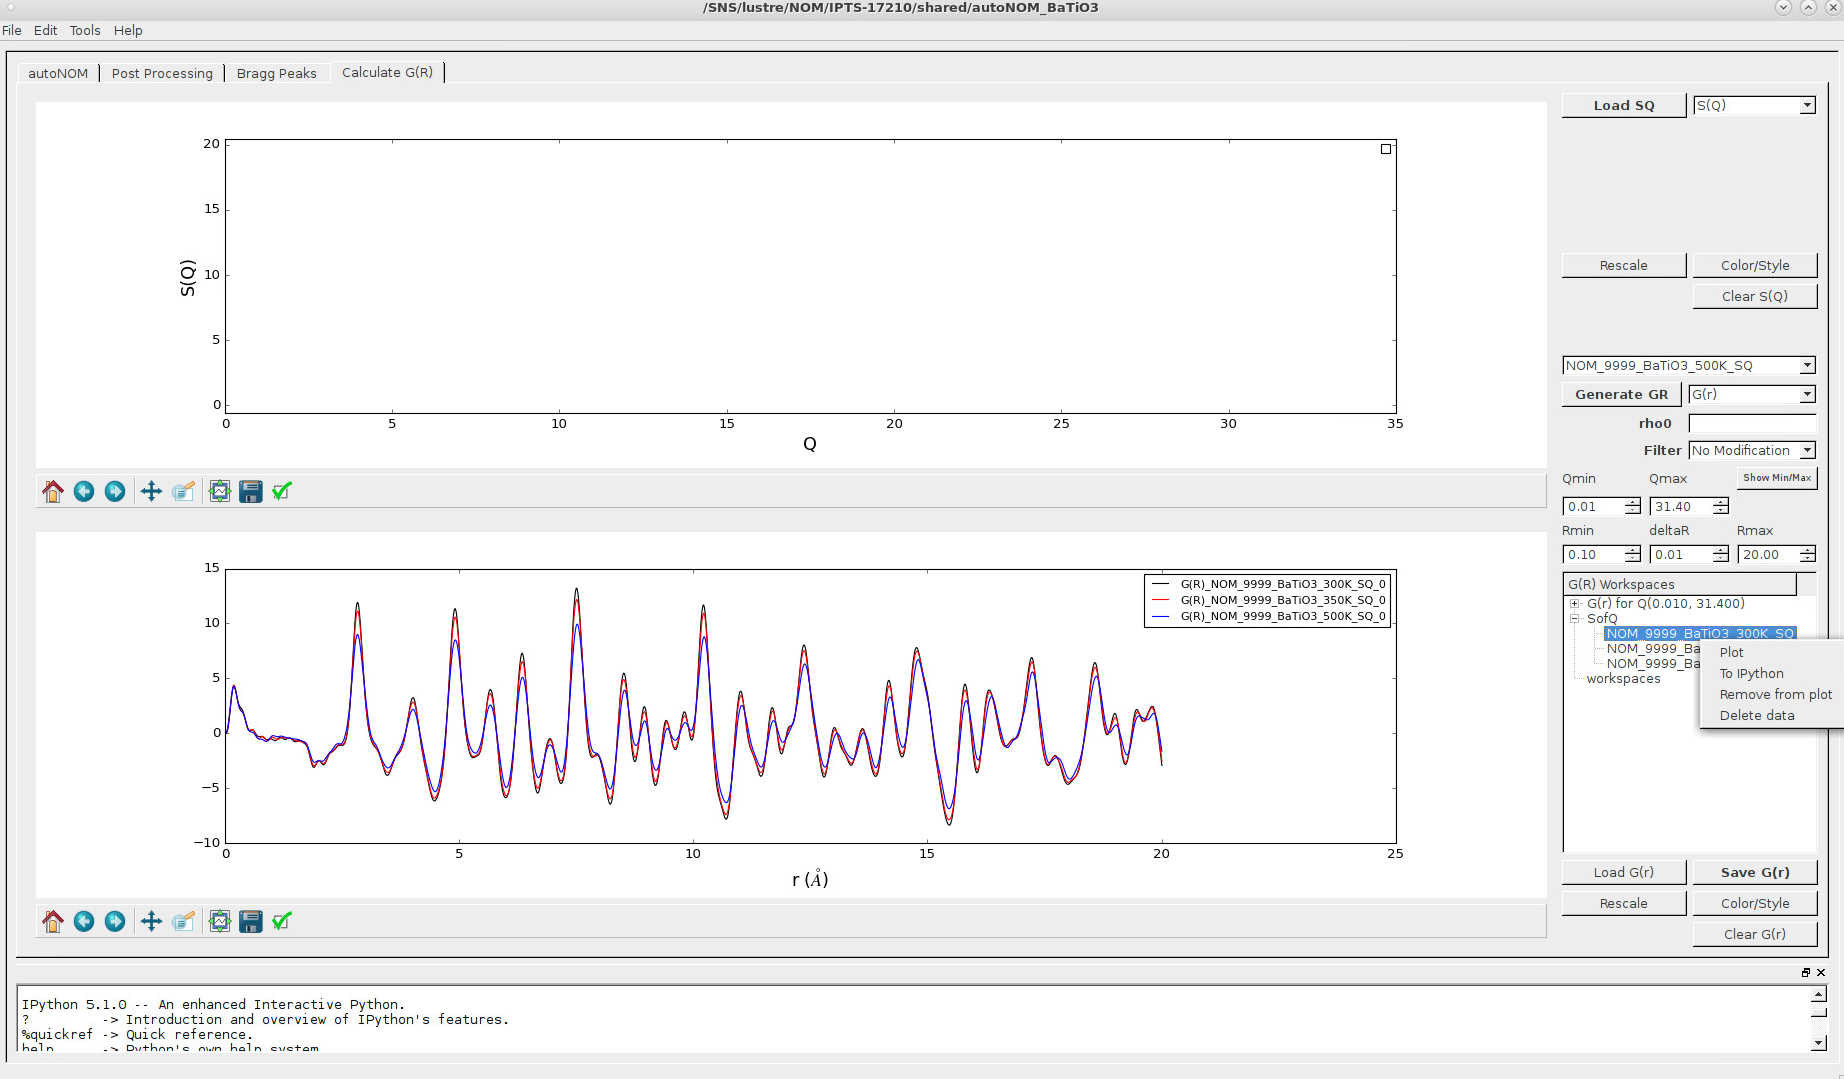
\includegraphics[width=0.9\paperwidth]{graphics/tab4/tab4_populatedGraph_workspaceTree_rightClick.png}}

These options are as follows:
\begin{itemize}

\item \guicmd{Plot}: This will plot the dataset in the S(Q) plot view.
\item \guicmd{To IPython}: Transfer the workspace to the IPython command line dock at the bottom. Here, you can script changes to the workspace and output a new workspace. If clicked, you will have something similar to what is shown below. Here, we have already typed in to add a 2.5 shift:

\noindent\makebox[\textwidth]{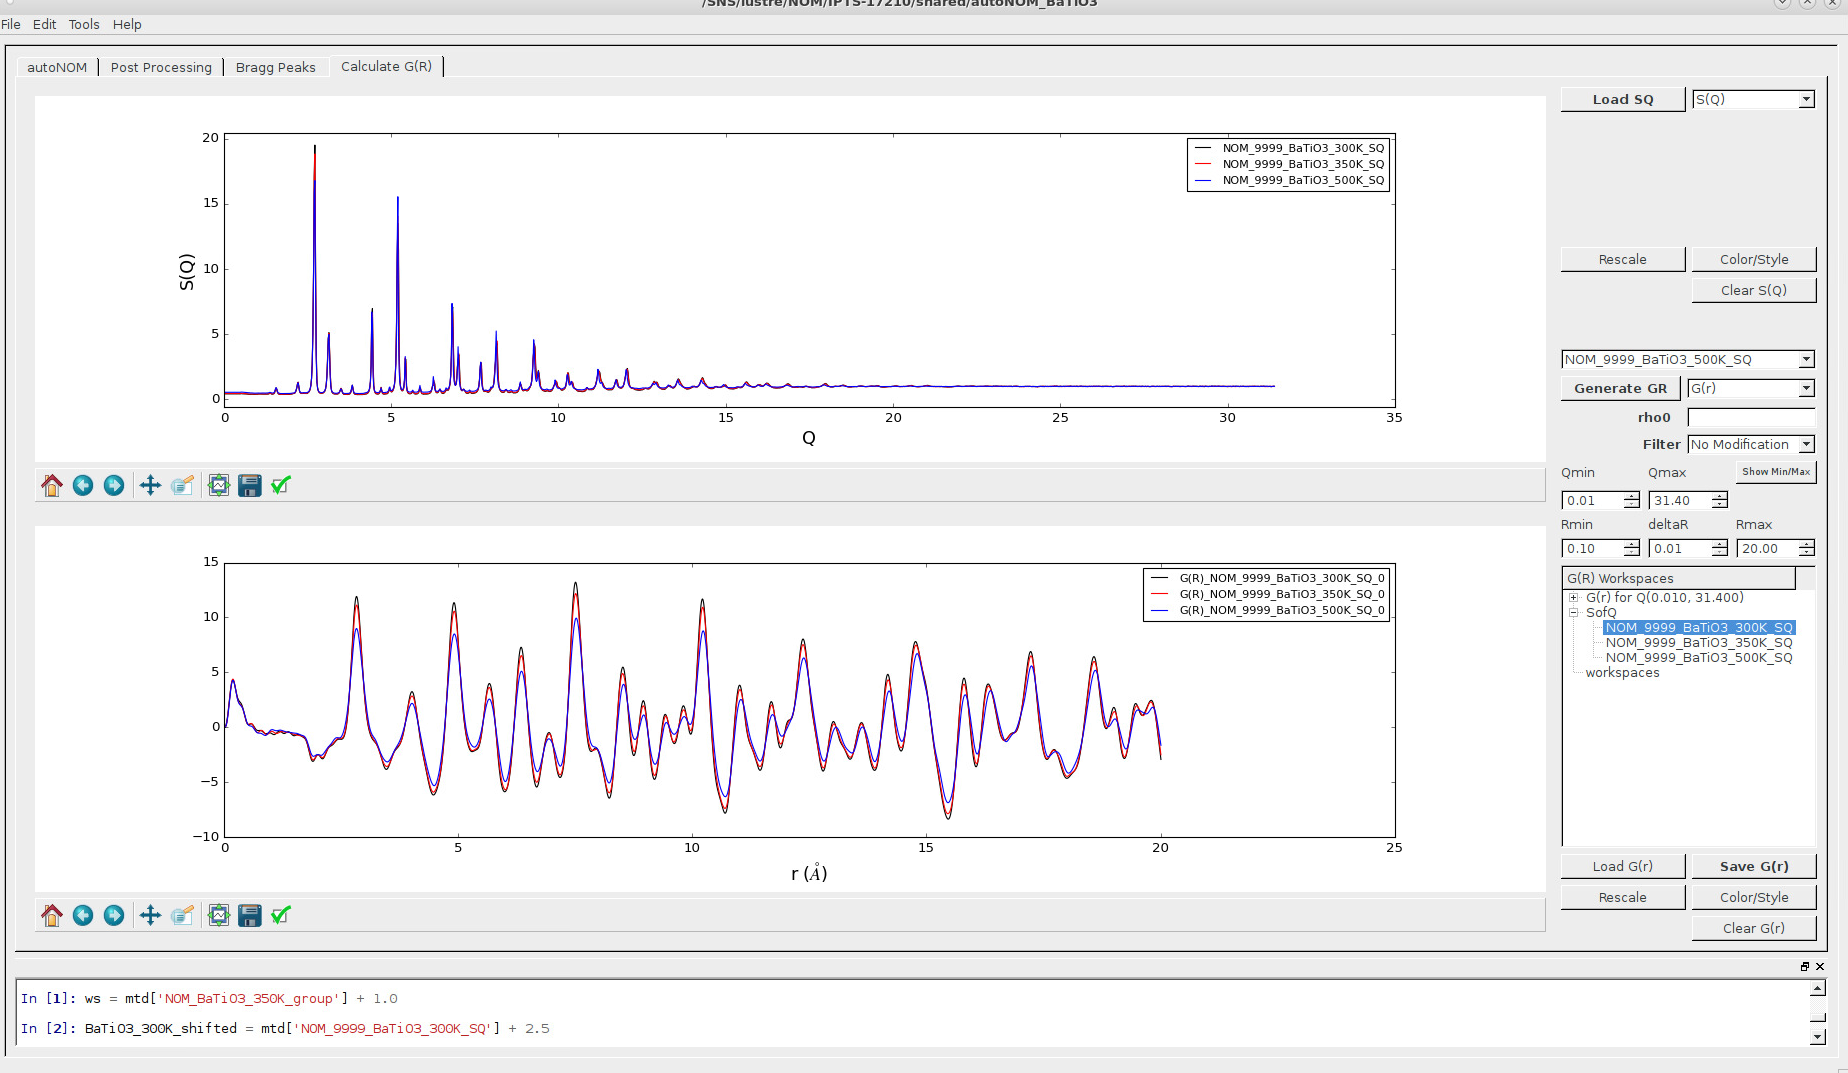
\includegraphics[width=0.9\paperwidth]{graphics/tab4/tab4_populatedGraph_workspaceTree_rightClick_ToIPython.png}}

If we name this new workspace "BaTiO3\_300K\_shifted" and execute the command in the IPython prompt, we will get a new SofQ workspace with this title in the \guicmd{Workspace Tree}. We show below the highlighted workspace in the tree and also have added the plot to the S(Q) plot area: 

\noindent\makebox[\textwidth]{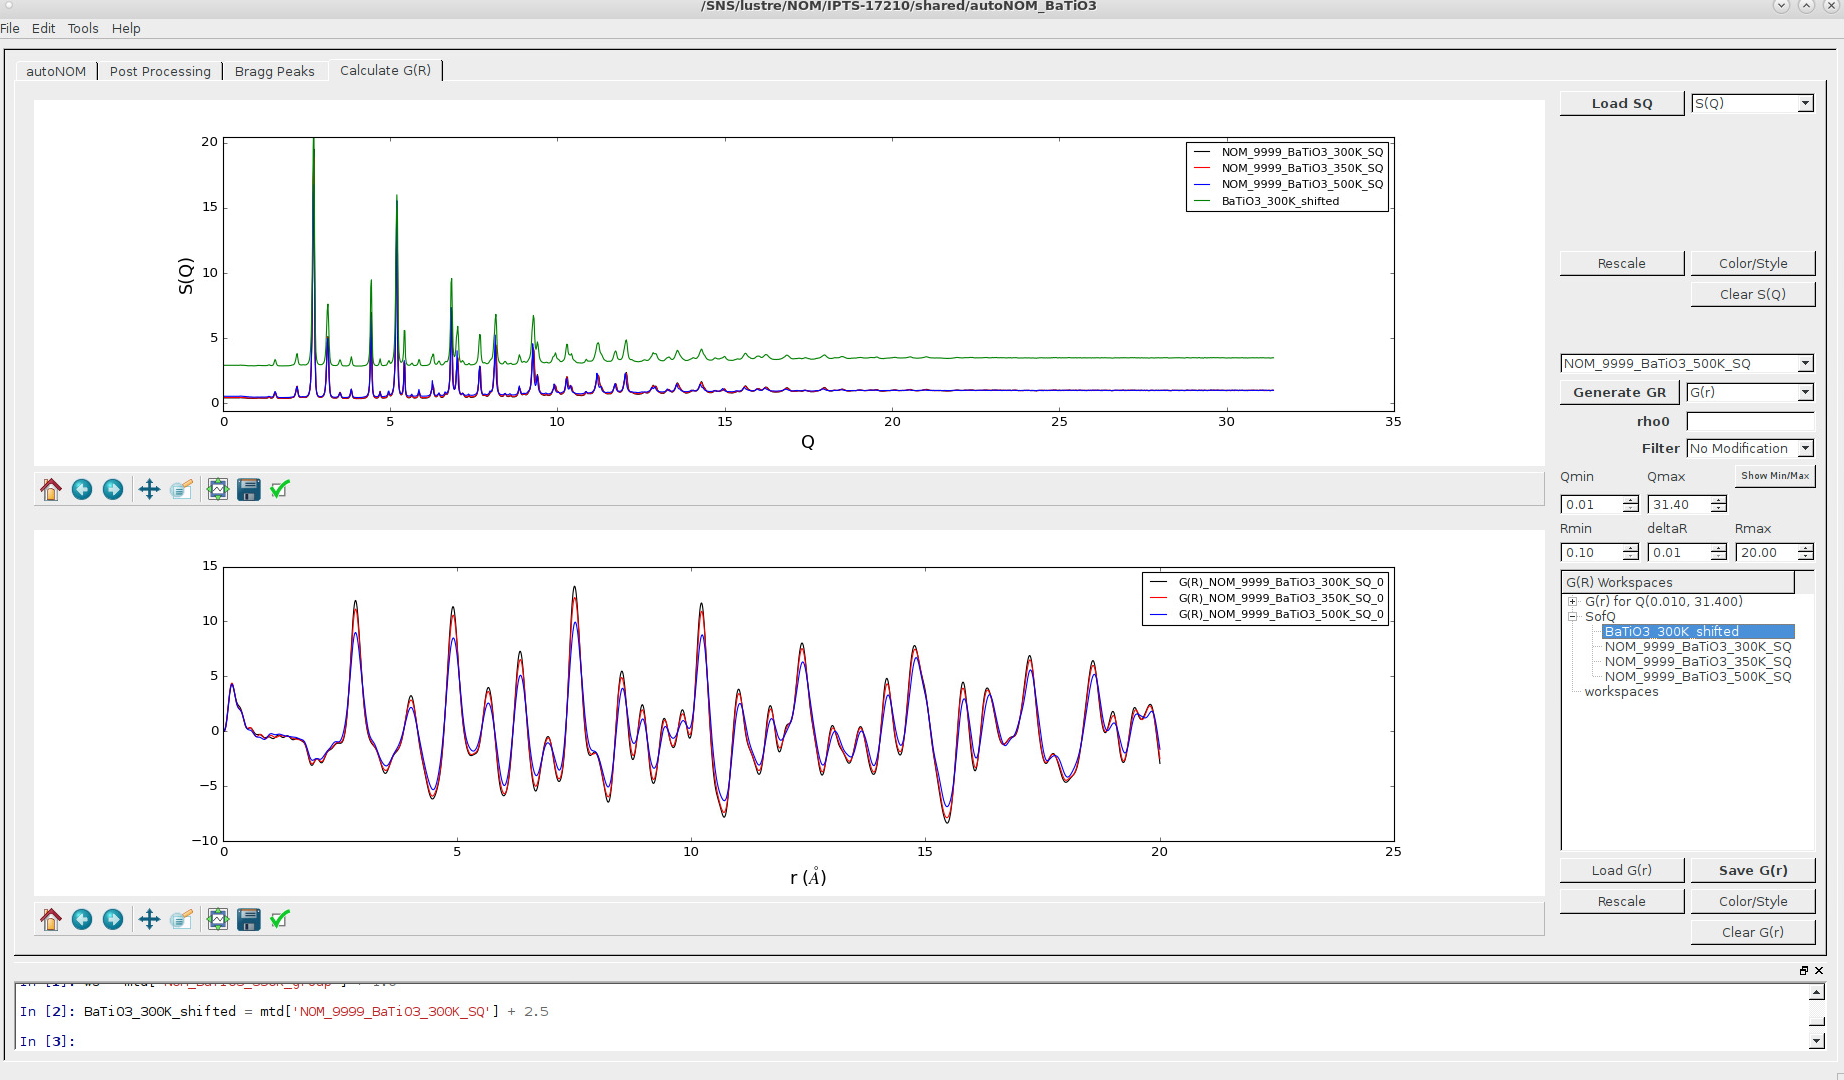
\includegraphics[width=0.9\paperwidth]{graphics/tab4/tab4_populatedGraph_workspaceTree_rightClick_ToIPython_addedToTree.png}}

You can dock and undock the IPython command line prompt by selecting the double-window icon on the top right of the dock, explained previously in the \guicmd{Bragg Peak} tab section.

\item \guicmd{Remove from plotting}: Removes dataset from the plot.
\item \guicmd{Delete data}: Deletes the dataset from the \guicmd{Workspace Tree}.

\end{itemize}

From the drop-down box above the \guicmd{Generate G(r)} button, we can select the new S(Q) workspace. Then, we can press the \guicmd{Generate G(r)} button to perform the Fourier transform on this S(Q) dataset. We see that the new G(r) dataset shows up as a workspace in the \guicmd{Workspace Tree} under the G(r) subtree. We show an example of this below:

\noindent\makebox[\textwidth]{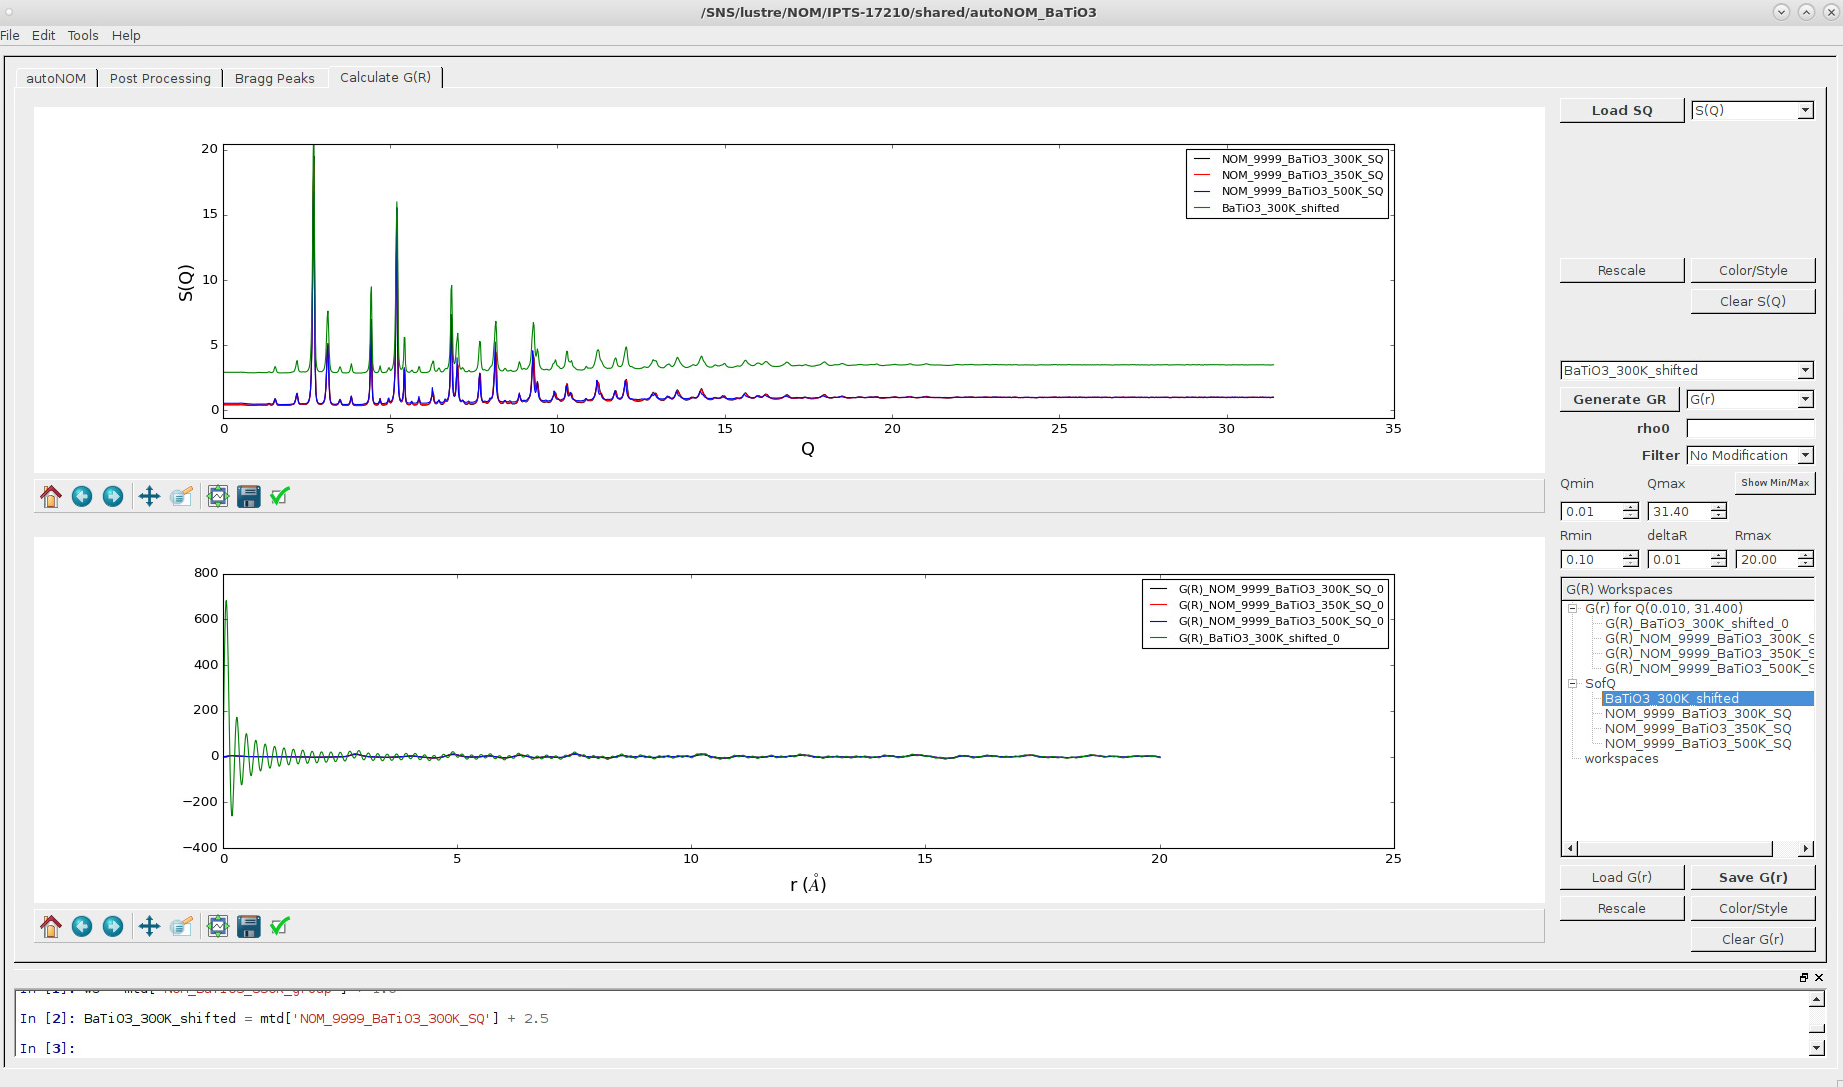
\includegraphics[width=0.9\paperwidth]{graphics/tab4/tab4_populatedGraph_workspaceTree_GofR.png}}

Also, from the drop-down beside the \guicmd{Generate G(r)} button, we can also select to generate \guicmd{g(r)} or \guicmd{RDF} (the Radial Distrbution Function).

If we right-click, we see that we have the same options for the G(r) workspaces as for the S(Q) workspaces:

\noindent\makebox[\textwidth]{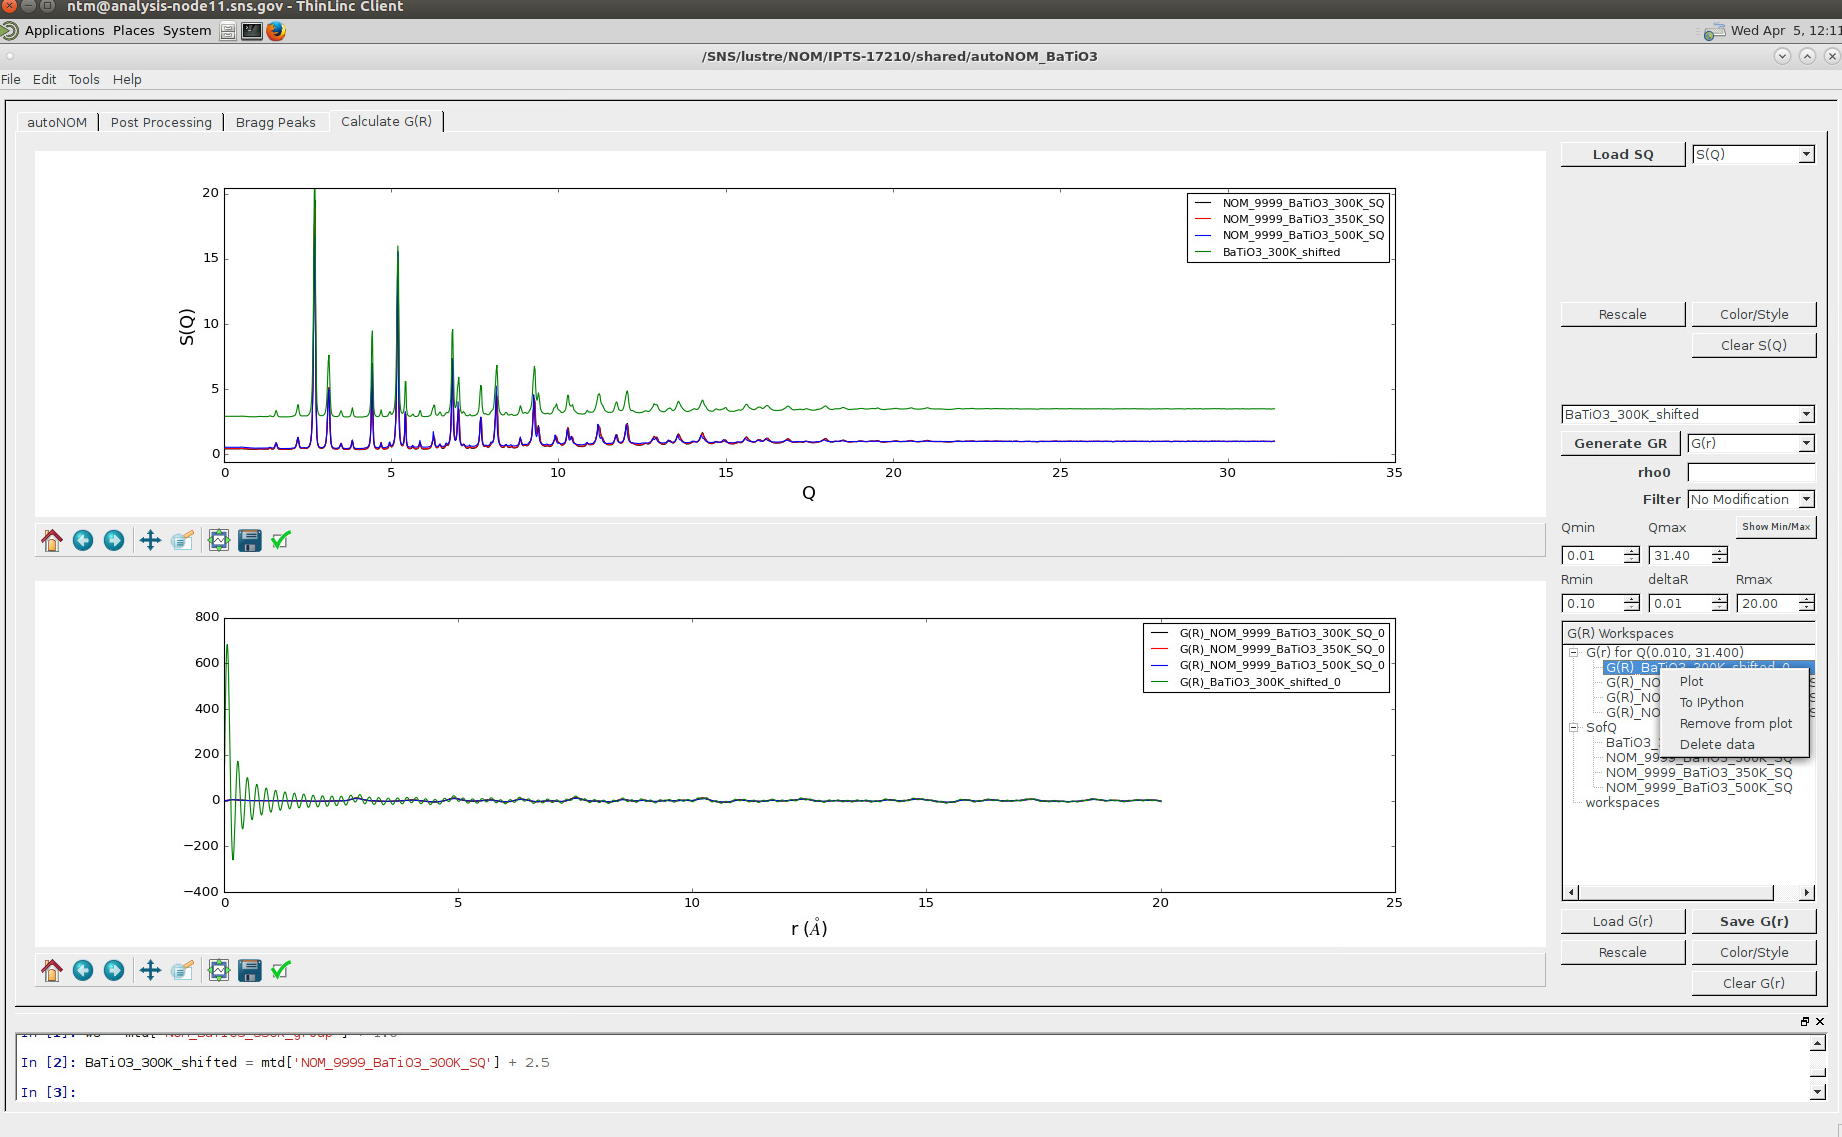
\includegraphics[width=0.9\paperwidth]{graphics/tab4/tab4_populatedGraph_workspaceTree_GofR_rightClick.png}}

Below, we have removed the G(r) workspace that was just created from the plot(the \guicmd{G(r) BaTiO3\_300K\_shifted\_0} workspace). Notice, it still exists in the \guicmd{Workspace Tree}:

\noindent\makebox[\textwidth]{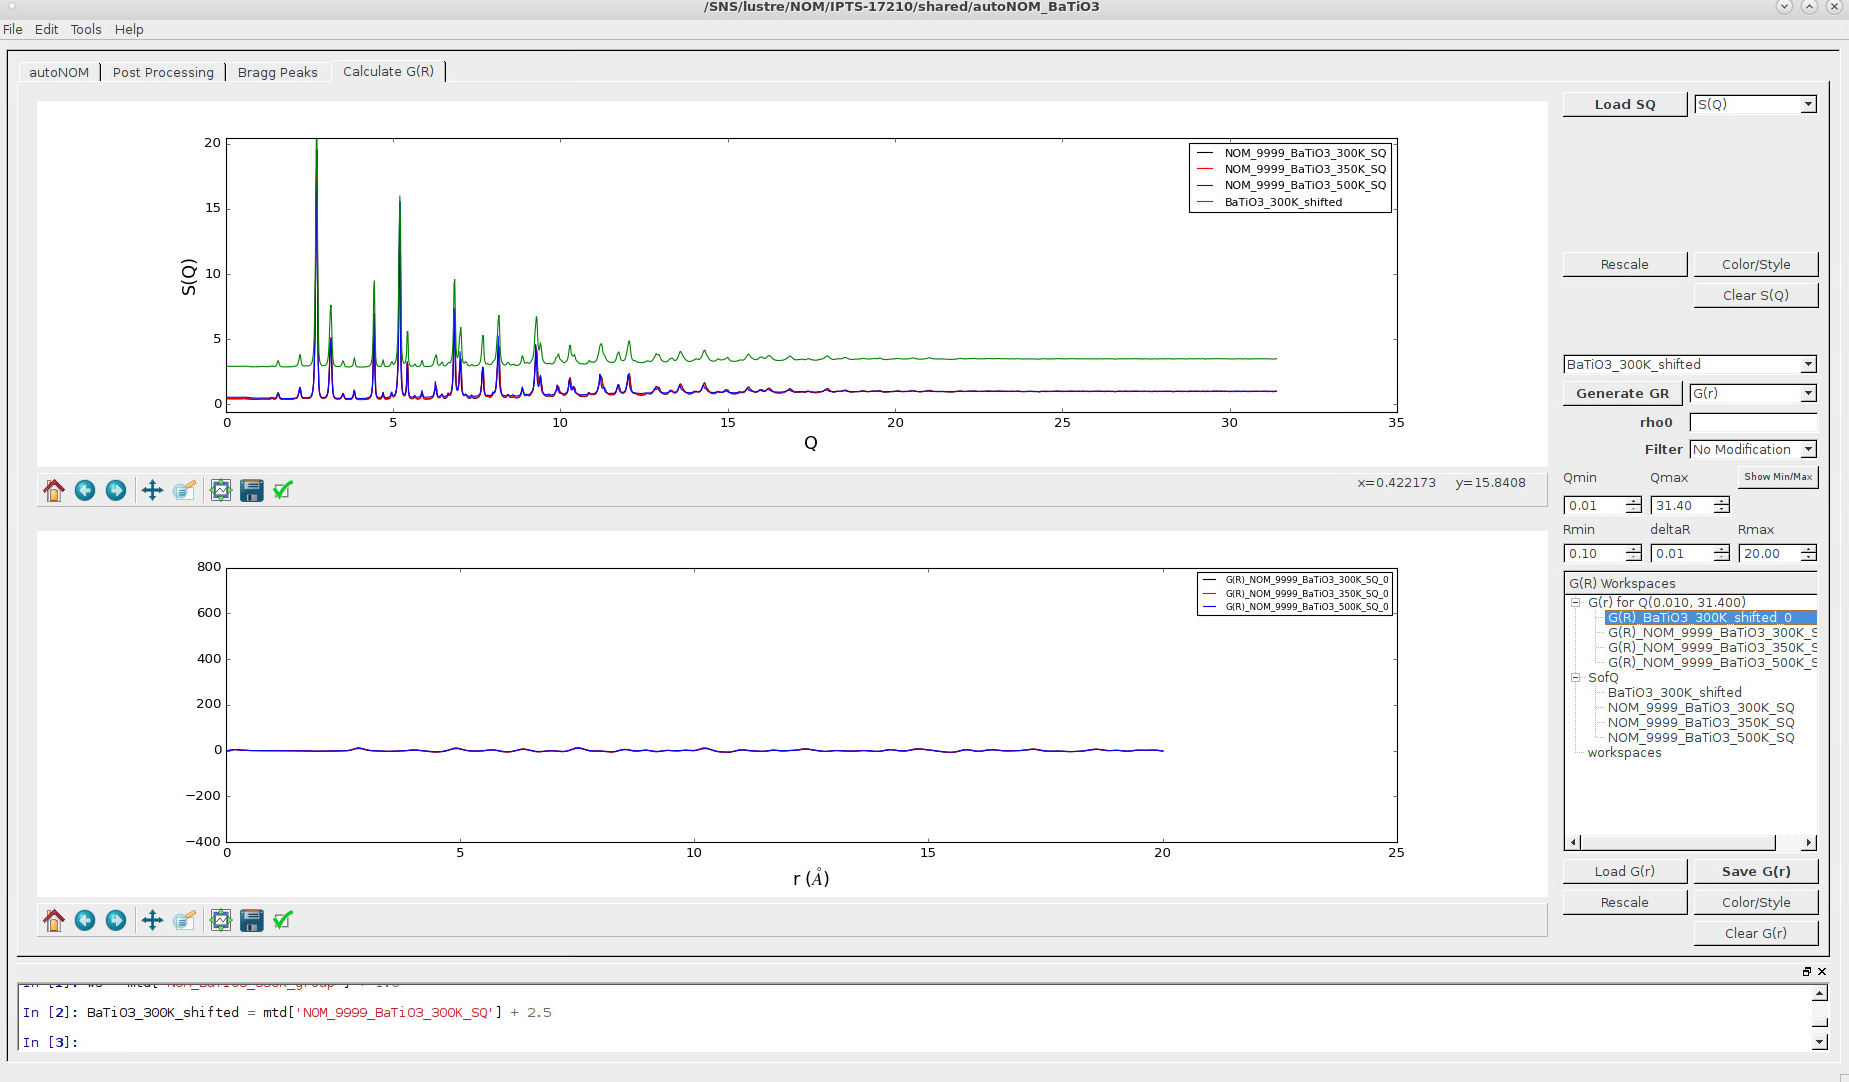
\includegraphics[width=0.9\paperwidth]{graphics/tab4/tab4_populatedGraph_workspaceTree_GofR_rightClick_removeFromPlot.png}}

Now, we can also delete the G(r) workspace.. Notice, it no longer exists in the \guicmd{Workspace Tree}:

\noindent\makebox[\textwidth]{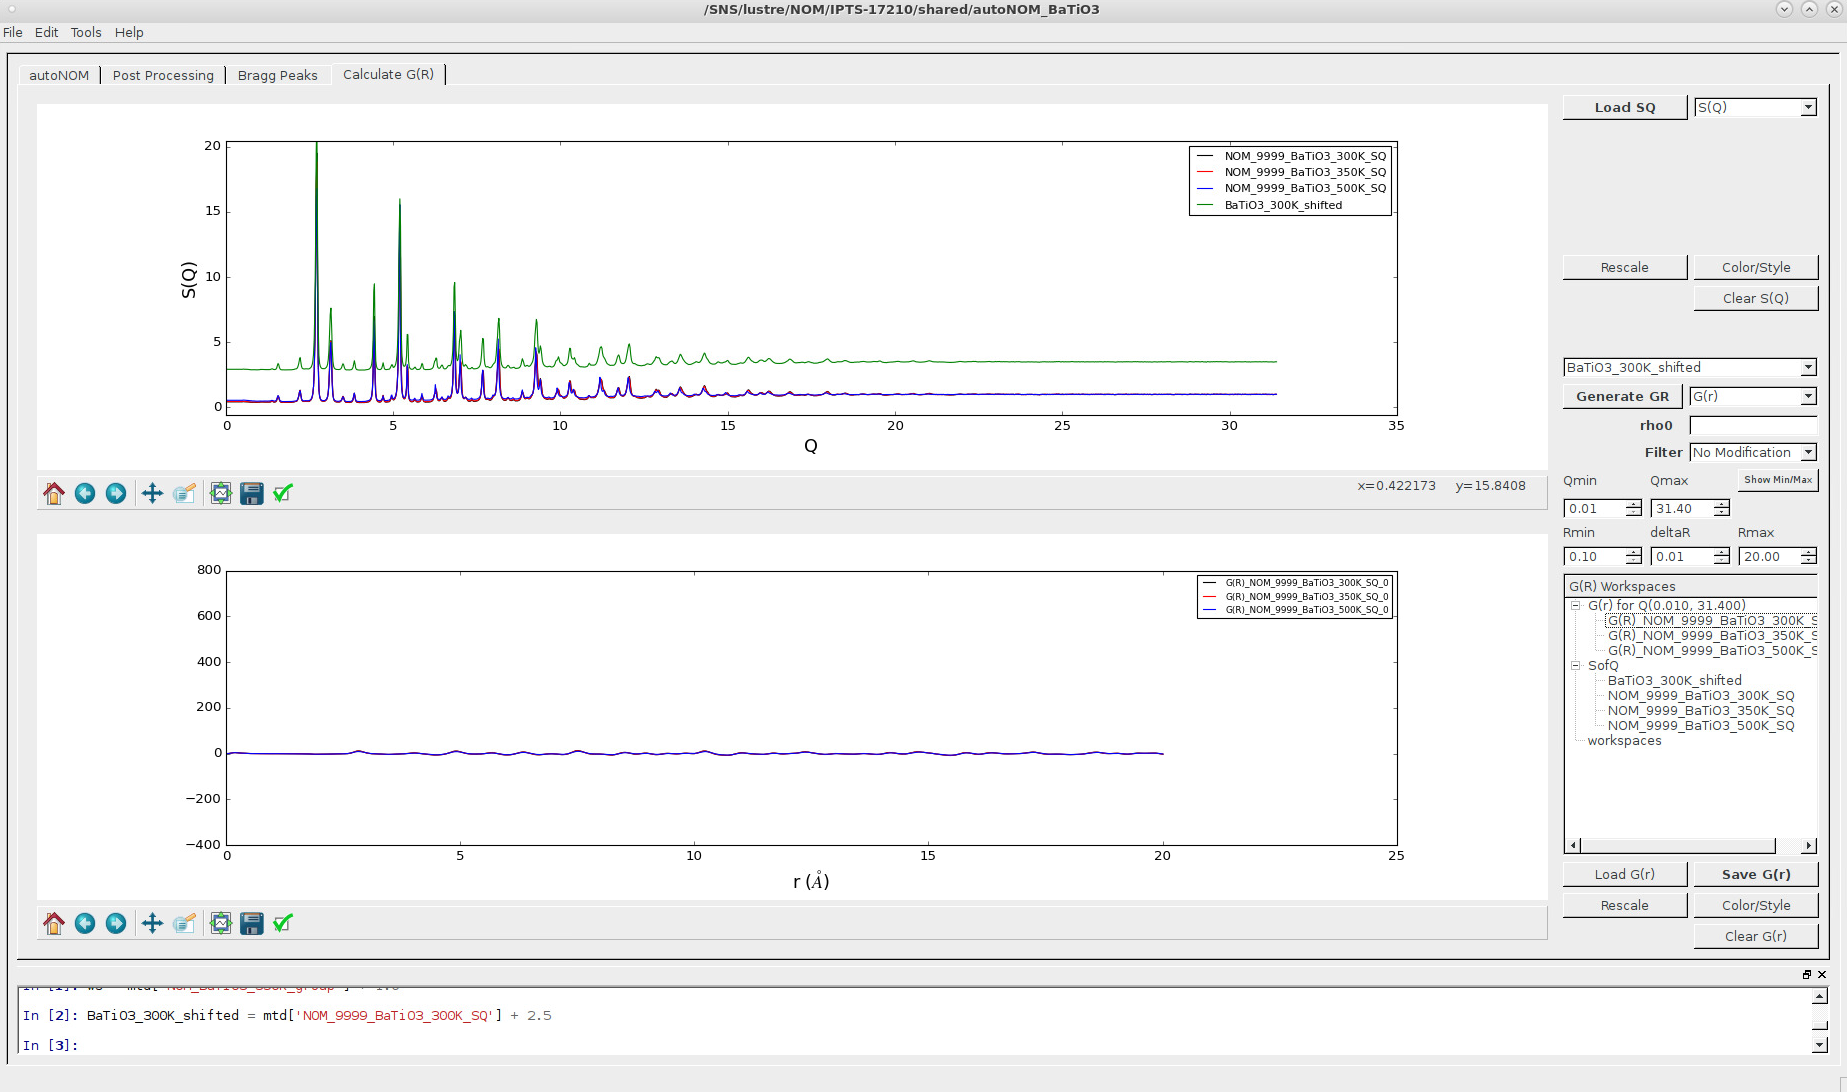
\includegraphics[width=0.9\paperwidth]{graphics/tab4/tab4_populatedGraph_workspaceTree_GofR_rightClick_deleteData.png}}

The \guicmd{rho0} field is used to input a bulk density value.

The \guicmd{Filter} drop-down is used to select different function we can use to transform and modify our data. Currently, the options are to apply no such function,  \guicmd{No Modification}, or to use the \guicmd{Lorch} function. Multiplication with a Lorch function reduced the influence of high Q noise and leads to smoother G(r)/PDF data. However, this comes at the expense of real space resolution (multiplication in Q = convolution in r).

The \guicmd{Qmin} and \guicmd{Qmax} specify over what Q range to perform the Fourier transform to produce a G(r). If we press the \guicmd{Show Min/Max}, we get a visual display in the S(Q) plot area of these \guicmd{Qmin} and \guicmd{Qmax} values we are using. An example is shown below:

\noindent\makebox[\textwidth]{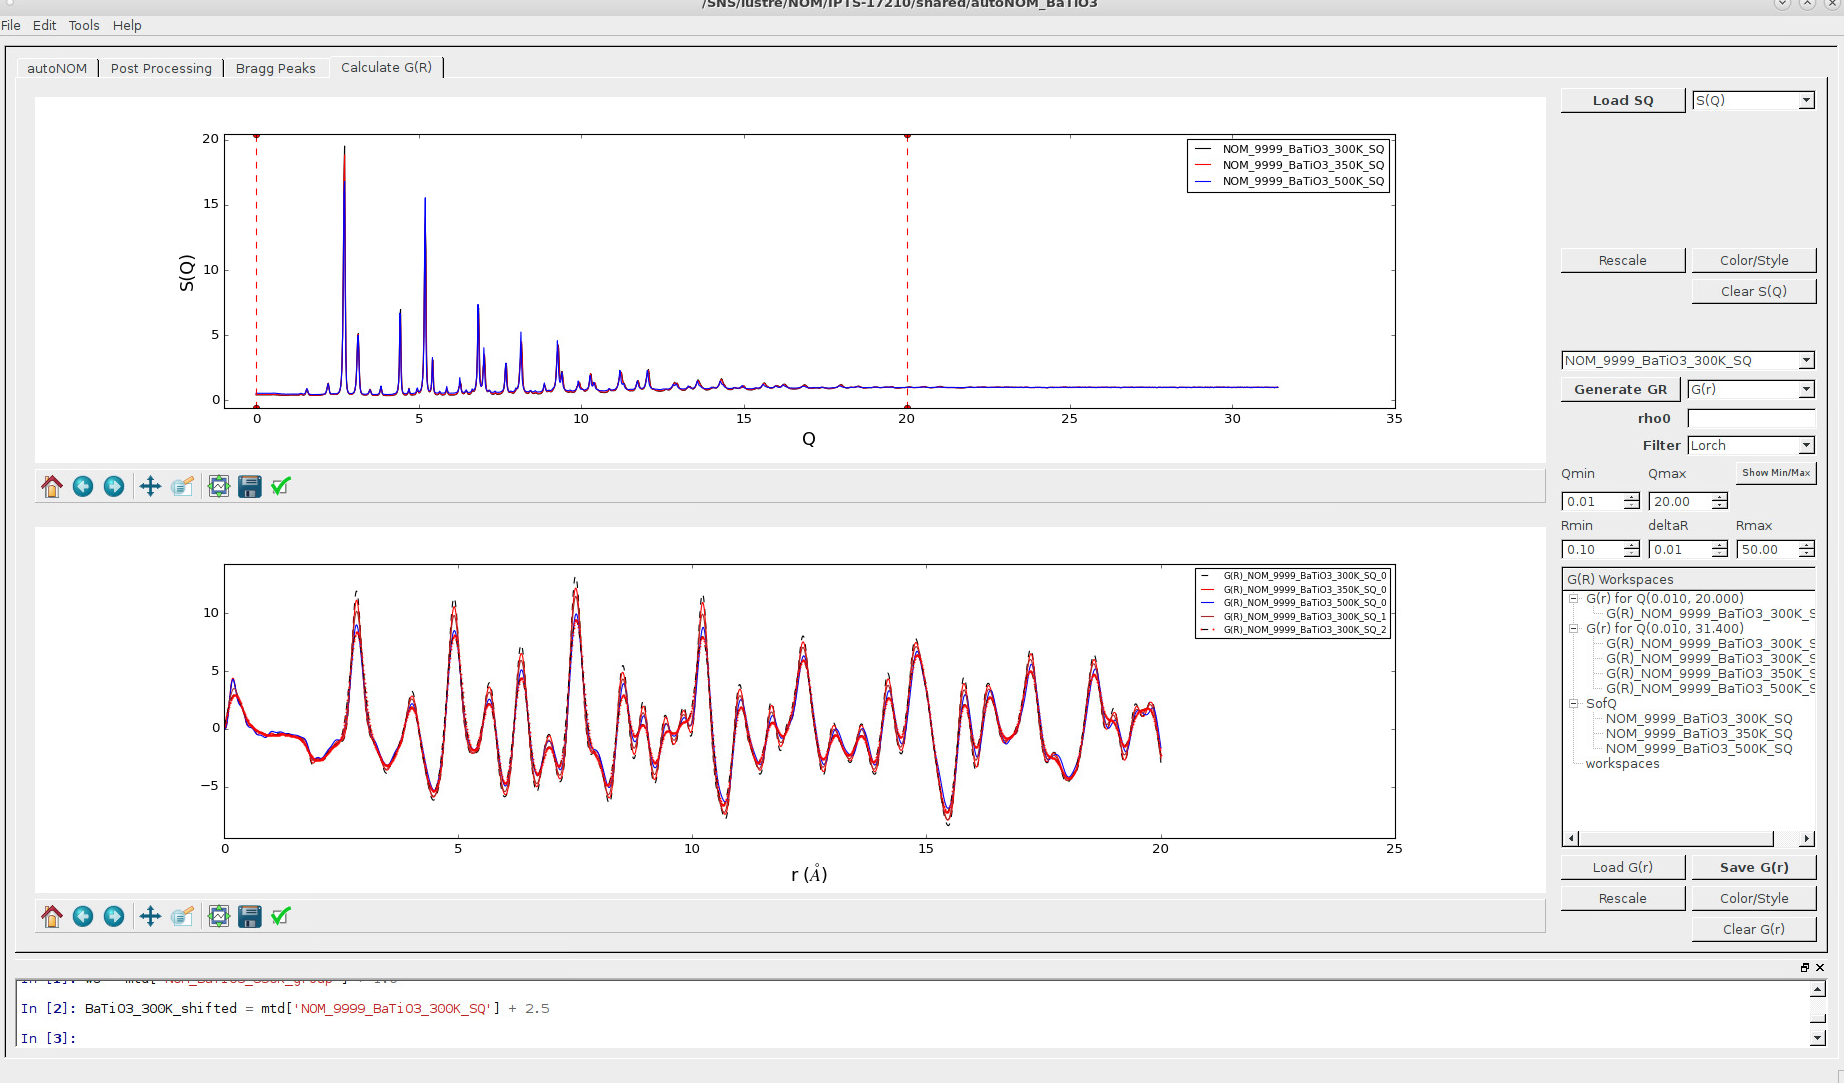
\includegraphics[width=0.9\paperwidth]{graphics/tab4/tab4_populatedGraph_differentQmaxTree.png}}

The \guicmd{Rmin} and \guicmd{Rmax} specify the minimum and maximum value of the real space data, respectively. The \guicmd{deltaR} specifies the bin size used for the produced G(r). Below, we show where we have extended the Rmax range for the G(r) produced:

\noindent\makebox[\textwidth]{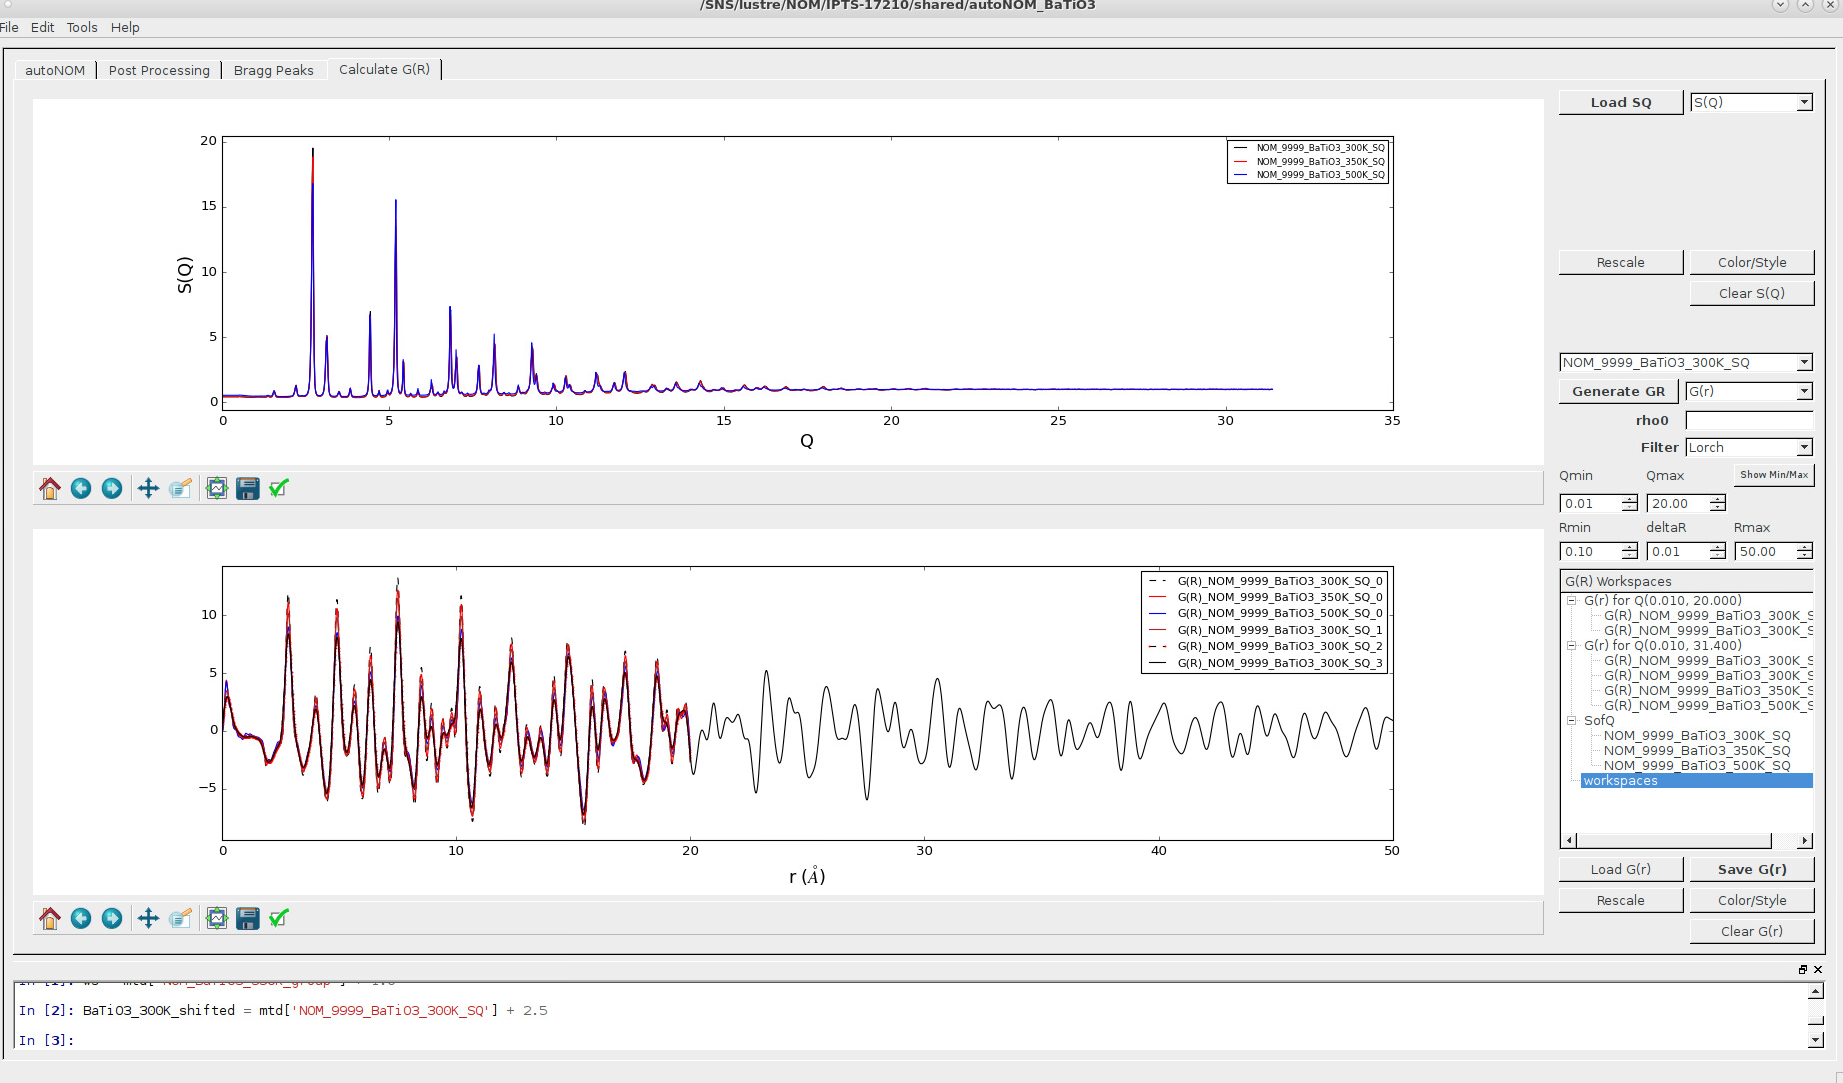
\includegraphics[width=0.9\paperwidth]{graphics/tab4/tab4_populatedGraph_extendedRMax.png}}

To change the legend, in case it is in the way or masking data, you can right-click inside any of the plot areas and either reduce the font of the text, increase the font of the text, or hide the legend all together. An example is shown below:

\noindent\makebox[\textwidth]{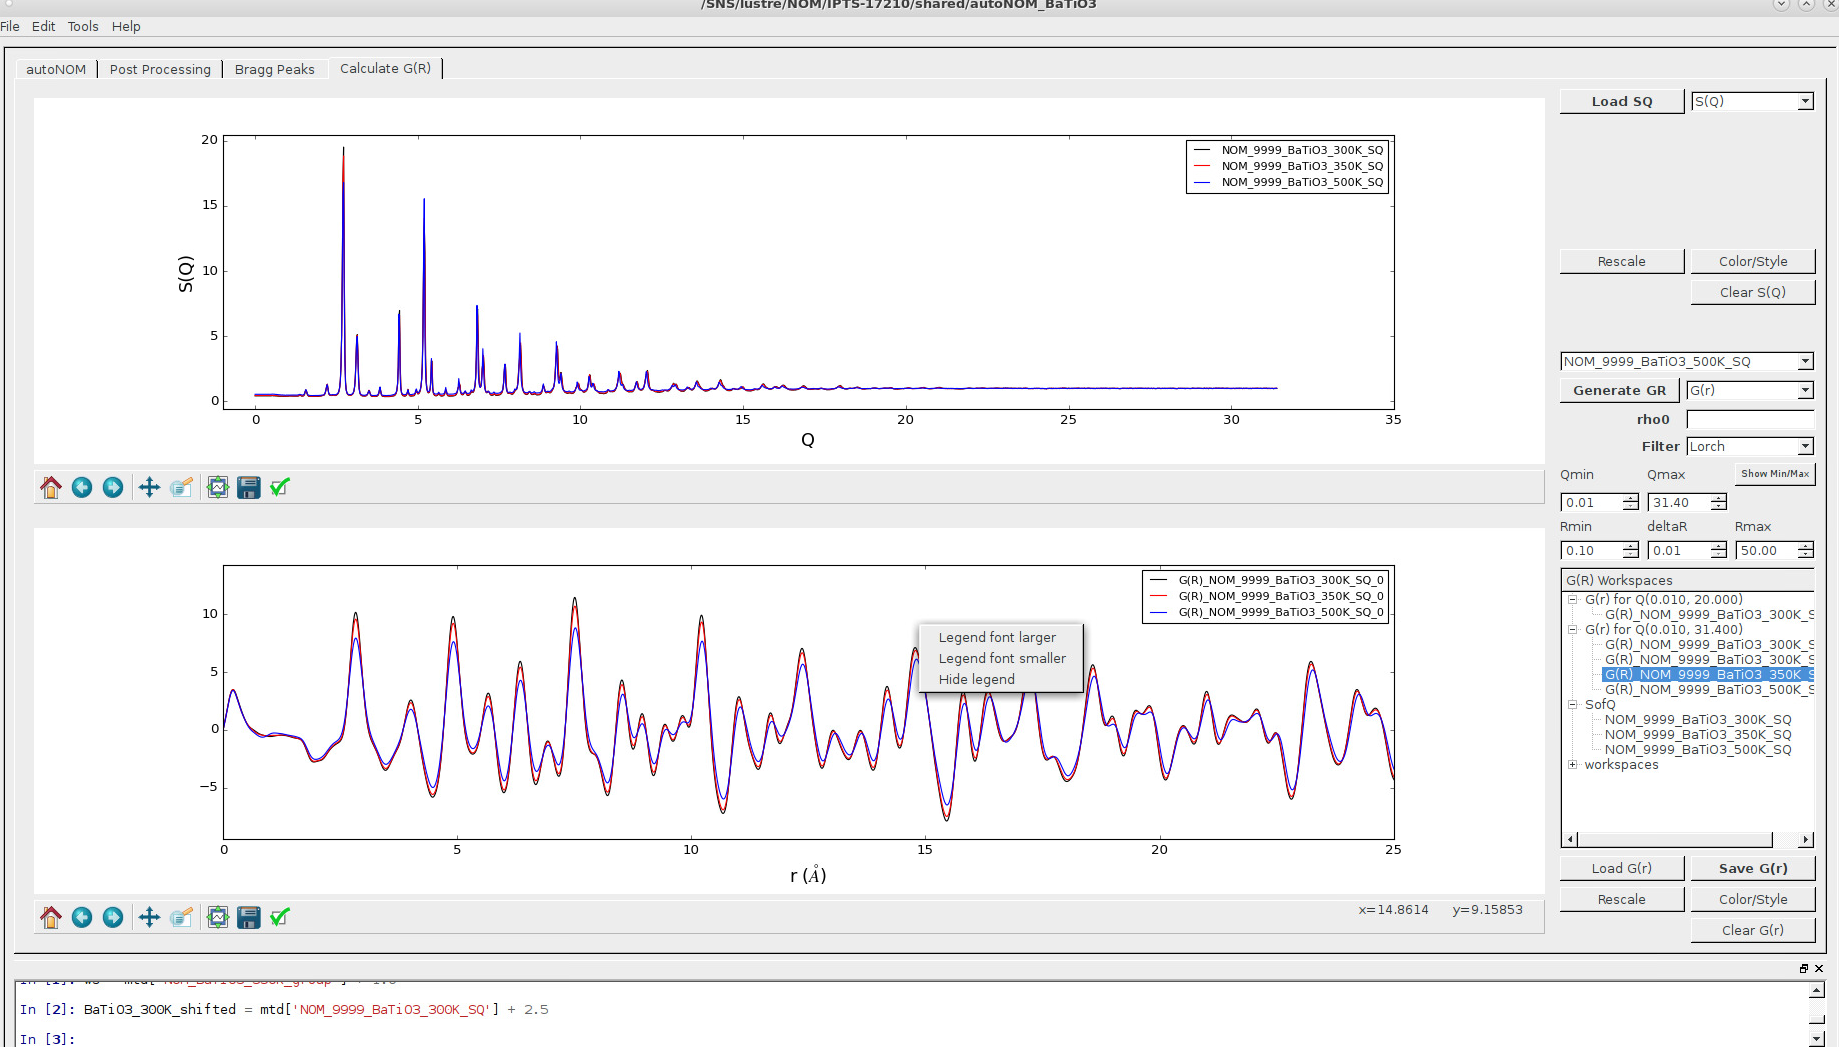
\includegraphics[width=0.9\paperwidth]{graphics/tab4/tab4_populatedGraph_rightClick_legendOptions.png}}

\subsection{Load G(r) data}
We can also load in our real space data from the individual runs or post-processed runs that are complete.  Go to the bottom right and press the \guicmd{Load G(r)} button. You can select either the \fileio{gofr} or the \fileio{PDF} file directories. 

If you choose the \fileio{PDF}, you should be presented with a file dialog similar to the one below:

\noindent\makebox[\textwidth]{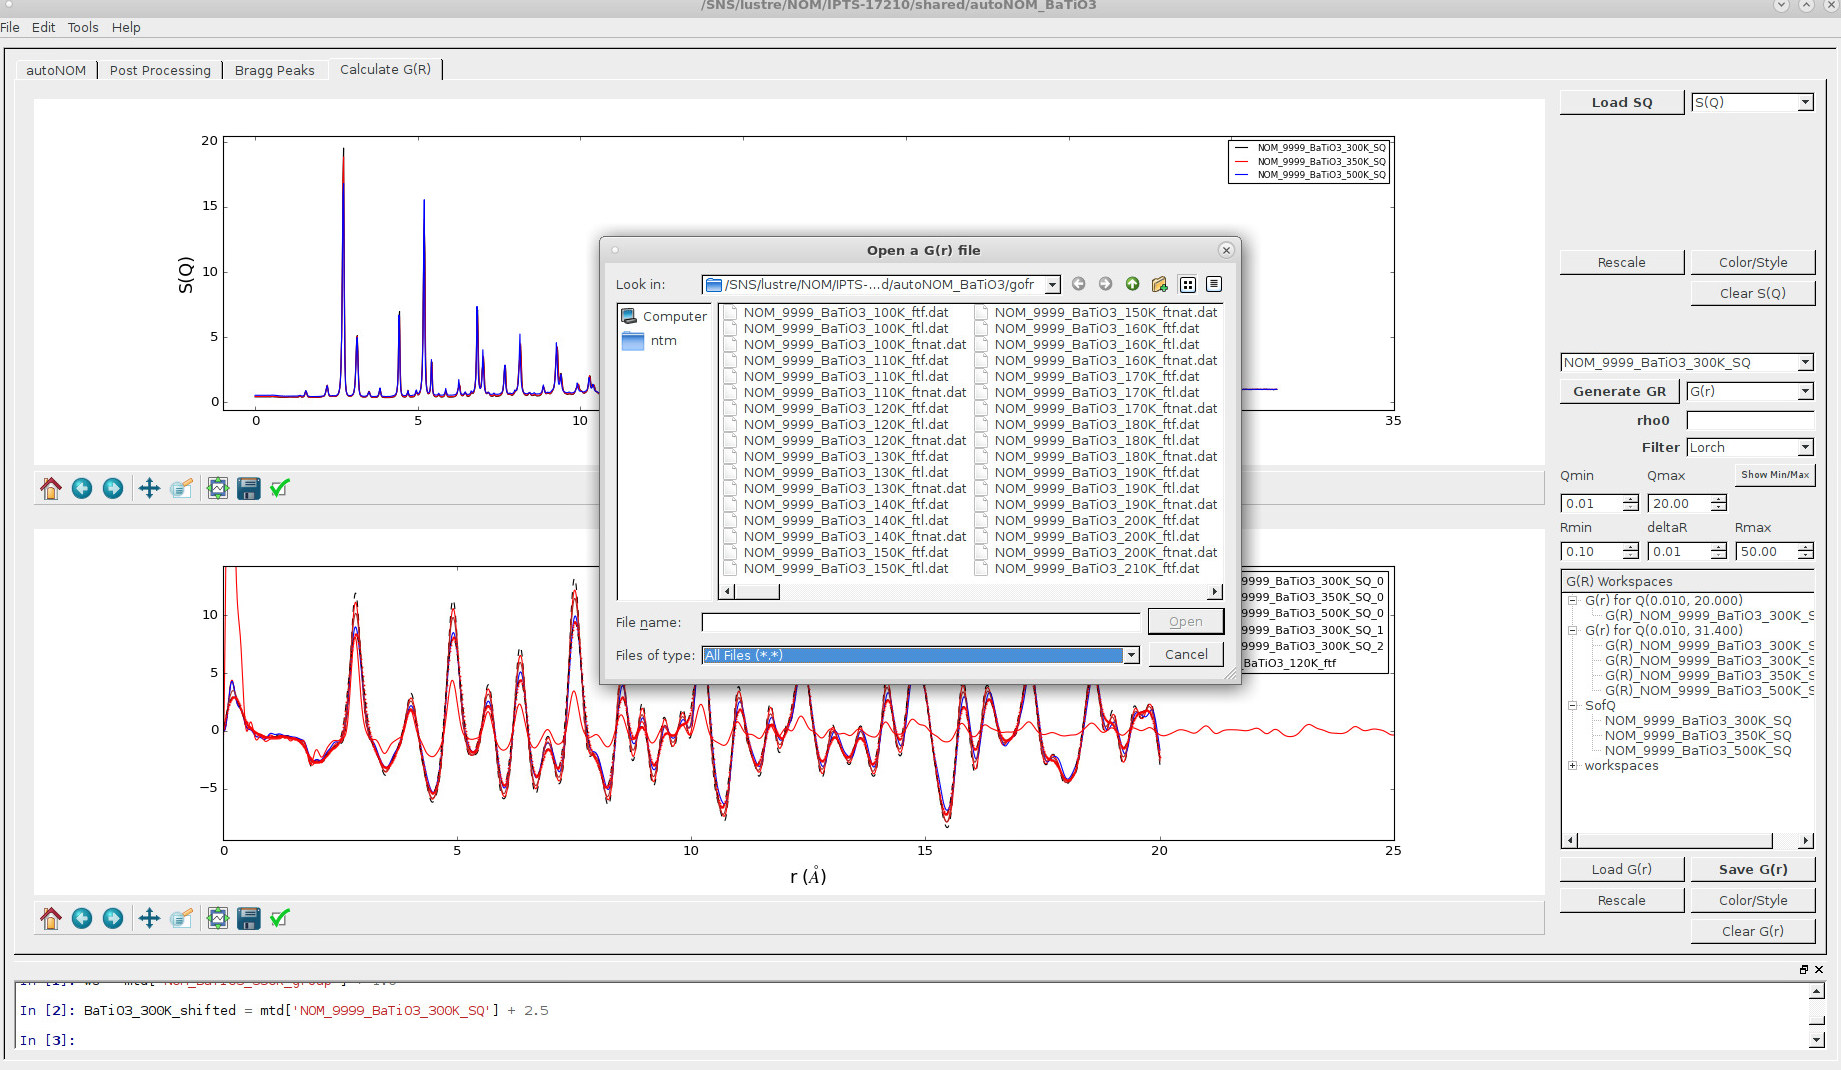
\includegraphics[width=0.9\paperwidth]{graphics/tab4/tab4_populatedGraph_loadGofR.png}}

If you choose the \fileio{gofr}, you should be presented with a file dialog similar to the one below:

\noindent\makebox[\textwidth]{\includegraphics[width=0.9\paperwidth]{graphics/tab4/tab4_populatedGraph_loadGofR_gofr.png}}

For the different file types of both, we have the following:

\begin{itemize}

\item NOMXXXftfrgr.gr – G(r) or PDF of your samples, ready for
analysis for PDFgui software package

\item NOMXXXftlrgr.gr – the same, but convoluted with the
Lorch function 

\item NOMXXXftl.dat, NOMXXXftf.dat – small g(r)

\end{itemize}


\subsection{Output G(r)}
The \guicmd{Save G(r)} button will allow you to output your selected G(r) workspace into a variety for file formats. Currently, you can output it to the following formats:

\noindent\makebox[\textwidth]{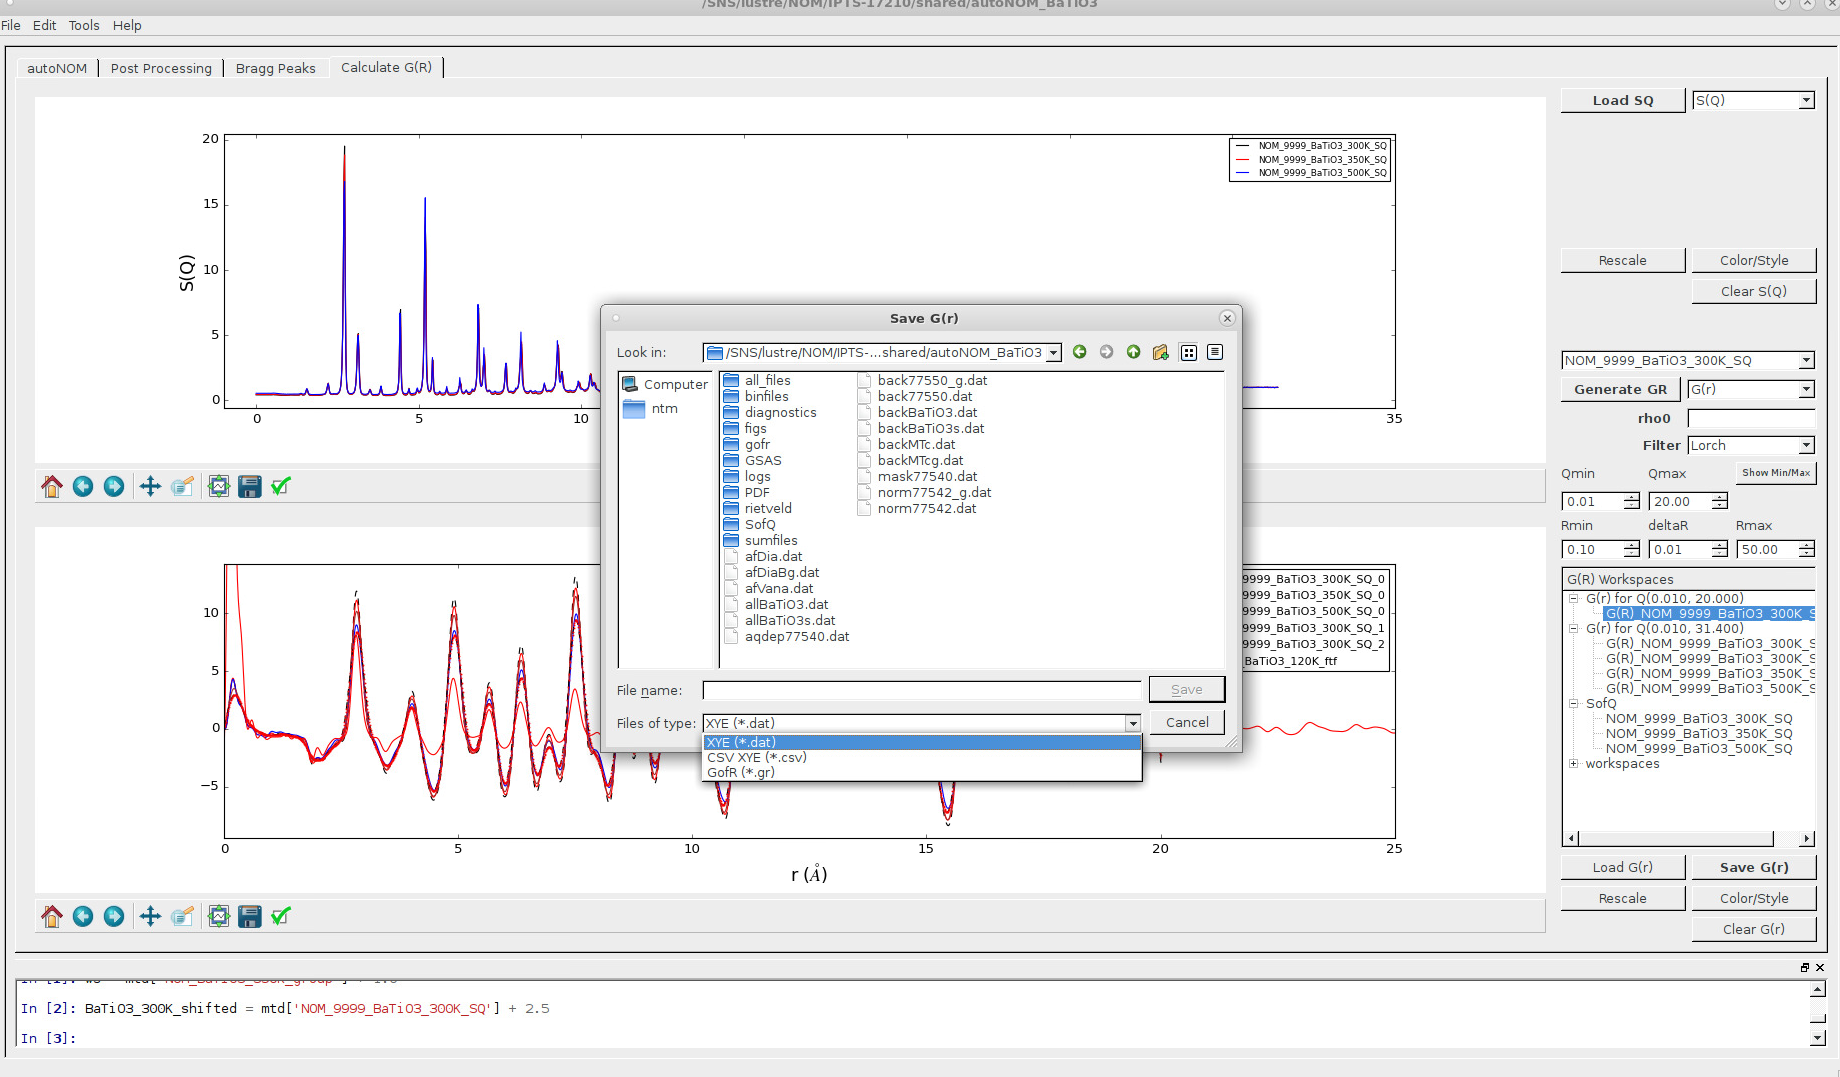
\includegraphics[width=0.9\paperwidth]{graphics/tab4/tab4_populatedGraph_saveGofR.png}}


\subsection{Optimize G(r)}

\textbf{Insert the optimization strategies we have discussed for each instrument scientist's method}


